%%\documentclass{aaStyle/aa}
%\documentclass[referee]{aa}
\documentclass{aa}
\usepackage{graphicx}
\usepackage[intlimits,sumlimits]{amsmath}
\usepackage{deluxetable}
\usepackage{times,epsfig} 
\usepackage{natbib}
\usepackage{amssymb}
\bibpunct{(}{)}{;}{a}{}{,} % to follow the A&A style
%for the bibliography at the end
\bibliographystyle{aa} %style aa.bst
\usepackage{amsmath}
\usepackage[english]{babel}

%-------------
\newcommand{\beqa}{\begin{eqnarray}} 
\newcommand{\eeqa}{\end{eqnarray}}
\newcommand{\Abst}[1]{\;#1}
\newcommand{\bsub}{\begin{subequations}}
\newcommand{\esub}{\end{subequations}}
\newcommand{\beal}{\begin{align}}
\newcommand{\ealn}{\end{align}}
\newcommand{\Nif}{$\rm ^{56}Ni$} 
\newcommand{\Cif}{$\rm ^{56}Co$}
\newcommand{\Fif}{$\rm ^{56}Fe$}
\newcommand{\ksm}{${\rm km~s^{-1}~Mpc^{-1}}$}
\newcommand{\s}{M$_{\sun}$}
\begin{document}
%
\title{Nickel mass estimates of Type Ia Supernovae from NIR data: Test case for SN2014J and SN2006X
}


\titlerunning{$M_{^{56}Ni}$ for SNIa from NIR data}
\authorrunning{TBD}%Stritzinger \& Sollerman}
\author{\textbf{TBD}}%M.~Stritzinger\inst{1}
 	%\and J. Sollerman\inst{1,2}}


\institute{European Southern Observatory, Karl Schwarzschild Strasse 2, Garching bei Munchen, Germany, 85748 \\
\email{ @eso.org}
\and  \\
%\email{jesper@dark-cosmology.dk}
} 

\offprints{TBD}
%
%\date{Received 21 December 2006 / Accepted May 6 2007}
%
\abstract{}{To determine the relation between the amount of Nickel produced in SNIa and the timing of the second maximum and to  extrapolate Nickel mass values for highly reddened SNIa using this relation} %between $^{56}$Ni masses ($M_{Ni}$)  and the timing of the NIR second maximum ($t_2$)}
%To investigate the 
%behaviour of the `bolometric' light curve at late phases
%of the normal type Ia supernova SN~2001el with the intent to understand
%the deposition of positron kinectic energy.}}
{We measure the  (pseudo)-bolometric luminosity at peak and use it to derive a value of $M_{Ni}$ mass for a 'low-reddening' sample of objects from the literature in order to minimize effects from presuming a reddening law. }
{We find a strong correlation between the $M_{Ni}$ and $t_2$ in the $Y$ and $J$ bands and a weaker trend in the $H$ band. We use this empirical relation to derive $M_{Ni}$ for two test case SN with high extinction ($>$  1.2 mag). This allows us to have a $M_{Ni}$ value which is independent of the reddening law applied.}
{From our results we conclude that an empirical relation between $M_{Ni}$ and $t_2$ can allow us to infer the $M_{Ni}$ for highly reddened objects without an estimate of their total absorption. The results for SN2014J from this method correspond well with the values obtained from recent $\gamma$ ray observations, thus providing further evidence of the potency of this technique}
%Our observations of SN~2001el provides no 
%evidence for complete positron escape as suggested by hitherto studies, 
%which have assumed that the late-time
%bolometric light curve follows the optical light curves. 
%previously believed.}
%This has implications for our interpretation and understanding of many aspects
%of supernova physics. 


%%-----------------
\keywords{stars: supernovae: general } %
\maketitle
\section{Introduction}
\label{sec-intro}

Type Ia supernovae (SNe\,Ia) have been used as cosmological distance indicators and have provided first evidence for the accelerated expansion of the universe \citep{Riess1998,Perlmutter1999}. . Their potency as cosmological probes has led to dedicated efforts to understand the nature of these explosions to reduce effects from systematics in the constraints of the cosmological parameters. 

SNIa in the optical, however, require corrections using correlations between observables \citep{Phillips1993, Tripp1998} to improve cosmological parameter estimation. Recent studies of SNeIa  have indicated that the SNIa are much more uniform in  
. 
%un-necessary self citation
%For a recent review see \citep{Goobar2011}.


Observations of large samples of SNe\,Ia %in optical and near-infrared 
show that the peak luminosity in the optical is not uniform
\citep[e.g.][]{Phillips1993, Riess1996, Guy2005, Guy2007, Guy2010,
Jha2007}, leading to different bolometric luminosities for the objects 
\citep{Contardo2000} implying variations in the physical
parameters of the explosion, in particular the synthesised nickel mass
and the total ejected mass \citep{Stritzinger2006, Scalzo2014}.  The
correlation at optical wavelengths between peak luminosity and light
curve shape together with the determination of the absorption towards
the supernova are the key ingredients of the calibration of these objects prior
to their use as distance indicators (\cite{Phillips1993}).
%citation not relevant for this paper.
%citep[see][for the most recent evaluation of the available SNe\,Ia for
%cosmology]{Betoule2014}. 


At near infrared wavelengths SNeIa display a very uniform brightness
behaviour \citep{Elias1981, 
% this is a late time reference for IR light curves not directly relevant here.
%Elias1983, 
Meikle2000, K04a, K07}. The
scatter in the peak luminosity in these studies is  0.2
magnitudes, which, combined with the lower sensitivity of the IR to 
extinction by dust, has sparked increased interest in this wavelength
region. Statistically significant samples of SN~Ia light curves are thus becoming available
\citep{WV08, Contreras2010, Stritzinger2011, BN12} and have been used
to construct the first rest-frame near-infrared Hubble diagrams
\citep{Nobili2005,Freedman2009, Kattner2012, Weyant2014}. 

The light curve morphology in the infrared is markedly different from
that in the optical, with a pronounced secondary maximum in $IYJHK$
filters for 'normal' SNe\,Ia and a 'shoulder' in the $V$ and $R$ filter
light curves \citep{Elias1983, Leibundgut1988, Leibundgut2000,
Meikle2000, WV08, Folatelli2010}. \cite{Kasen2006} demonstrated that the
second maximum could be the result of decrease in opacity due to the
ionization change of Fe group elements from doubly to singly ionized
atoms, which preferentially radiate the energy at near-IR wavelengths.
He further indicated that larger iron mass would lead to a later maximum
in the NIR light curves.

Recent studies have shown a strong dependence of the timing of the second maximum (hereafter $t_2$)
on the decline rate of the SNIa, indicating that brighter explosions have a later onset of the second maximum. A strong relation
between the $t_2$ and the onset of the uniform optical colour phase \citep[hereafter $t_L$, see also $t_{max}$][]{Burns2014} suggests that the second maximum is related to the colour evolution
which is tied to the amount of iron group elements synthesized in the explosion (\cite{Kasen2007}). The conclusion from these studies point to a connection between 
the $M_{^{56}Ni}$ in SNIa and $t_2$. 

In this study, we investigate ,directly, the link between the  $M_{^{56}Ni}$ and $t_2$. We use a sample of nearby objects with low extinction from dust, in order to circumvent uncertainties
from the specific reddening law used. We aim to use this relation to derive $M_{^{56}Ni}$ for heavily extinguished SNae where using the bolometric peak is extremely sensitive to the 
total absorption value used, and hence, the reddening law. To this end, we propose using NIR only data at late times along with an empirical relation to obtain precise 
estimates of $M_{^{56}Ni}$ for objects where other methods provide disparate results. 


\iffalse
Dust extinction in the near-infrared is significantly reduced compared
to the optical leading to smaller corrections for dust and hence
decreased uncertainty introduced by these corrections. The optical dust
correction of SNe\,Ia is notoriously difficult and has led to large
discrepancies between individual supernovae and for complete samples. It
could even affect the light curve shapes for strongly reddened SNe\,Ia
\citep{Leibundgut1988, Amanullah2014}. Today, it remains unclear what
extinction law for the dust correction should be used \citep[see discussions in][]{Phillips2013, Scolnic2014} 
and this represents a major
uncertainty for the application of SNe\,Ia to cosmology
\citep[eg.][]{Peacock2006, Goobar2011}. The recent SN\,2014J is a case in
point with derived dust properties very different from local
interstellar dust \citep{Amanullah2014, Foley2014}. 




Studies of the $i$ band light curve find a relation between the phase
of the second maximum and the optical light curve shape 
\citep[e.g. $\Delta m_{15}(B)$, ][]{Folatelli2010, Hamuy1996}. The strength
of the second maximum in $i$ does not show such a correlation.

The properties of SNe\,Ia infrared light curves are investigated and
possible correlations with physical properties, e.g. nickel mass, are
established. The structure of this paper is as follows: after a
presentation of the input data in Section \ref{sec:data}, we analyse the
infrared light curve properties (Section~\ref{sec-LC}) along with a
description of IR colours. Correlations with optical light curve
parameters and their interpretations in section are given in
\S\ref{sec-corr} followed by a discussion in \S\ref{sec-disc}.

\fi


\begin{figure}
\centering
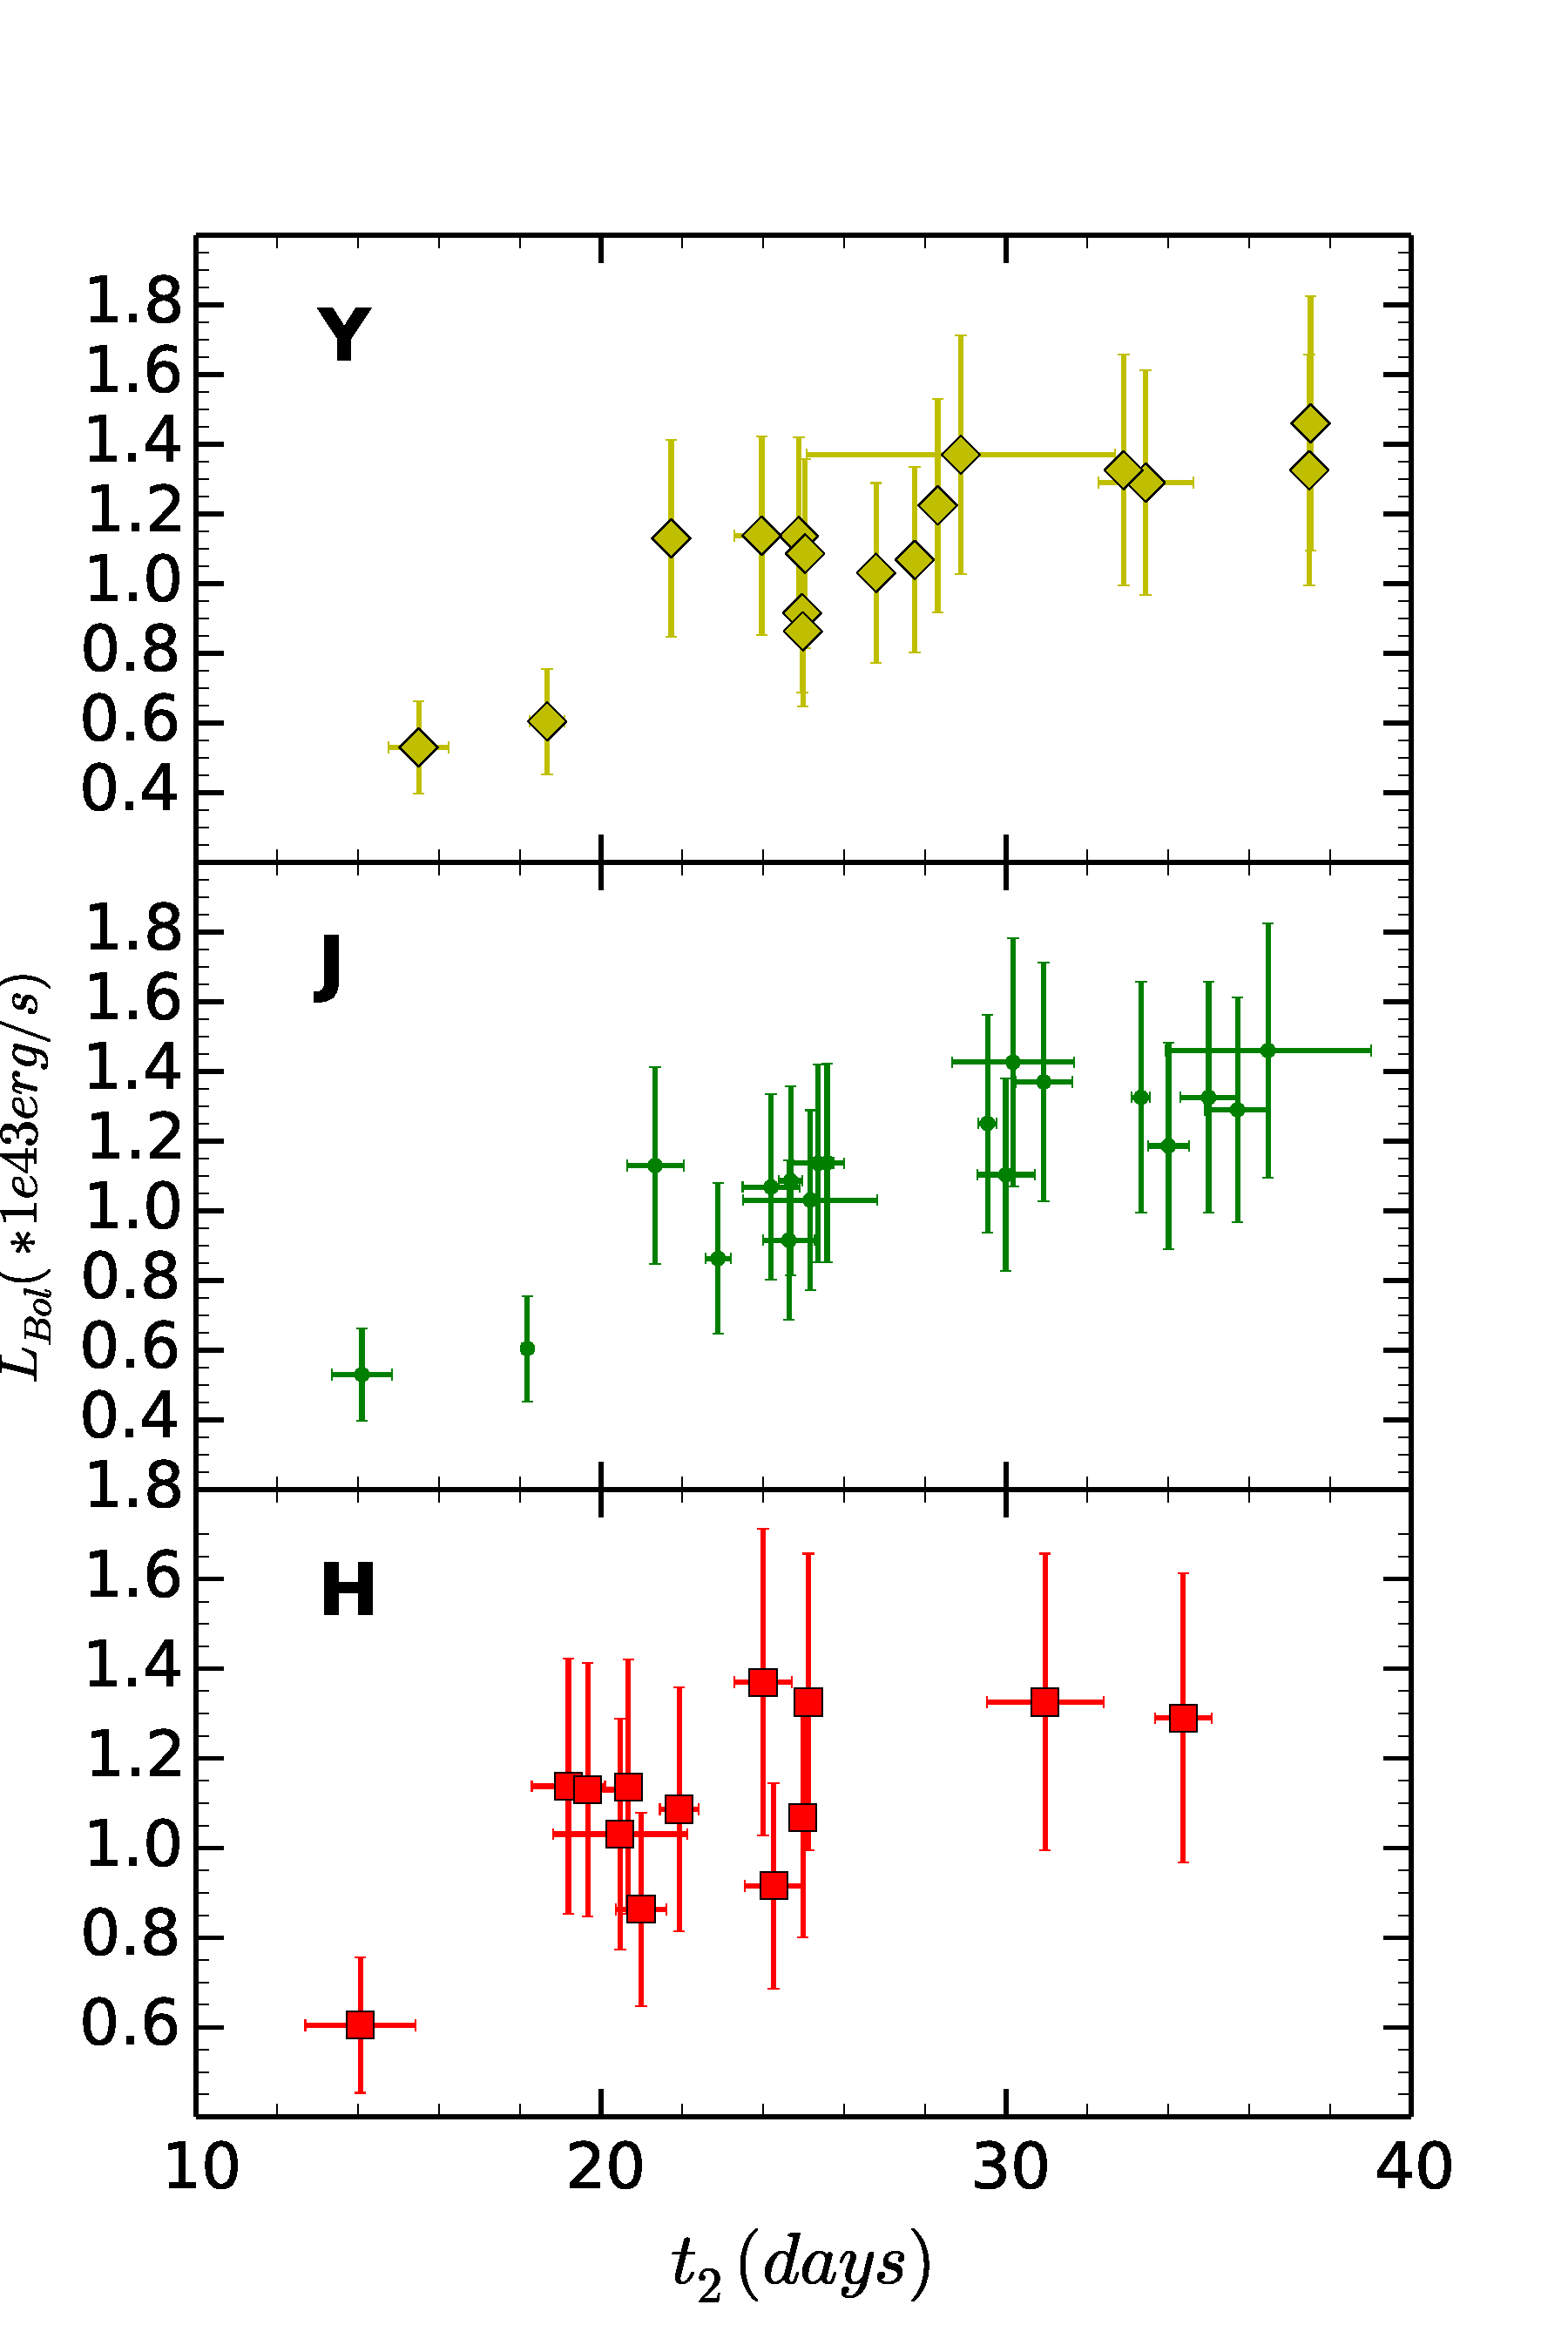
\includegraphics[width=.50\textwidth, height=0.6\textheight]{../plot_rel/t2lbol.pdf}
\caption{$L_{max}$ is plotted against the $t_2$ in $YJH$ bands. A strong correlation is observed in the $Y$ and $J$, whereas a weaker correlation is seen in the $H$ band. {\bf this only includes objects with a u-H measured bolometric peak and not any of the others}}
\label{fig:nit2}
\end{figure}



\section{Data} 
\label{sec:data}
%


The sample for this study is constrained by objects which have NIR observations at late times as well as well-sampled optical light curves to
construct a (pseudo-) bolometric light curve. The main data source of
near-infrared photometry of SNe\,Ia currently comes from the Carnegie
Supernova Project \citep[CSP;][]{Contreras2010,Burns2011,Stritzinger2011,Phillips2012,Burns2014}.
They form an ideal basis for an evaluation of light curves parameters.
We add to this sample objects from the literature and the nearby objects SN2011fe.


Since we aim to circumvent the uncertainties from host galaxy extinction, we only select objects with an $E(B-V)_host$ value
less than 0.1. Since we want to investigate the connection of $M_{Ni}$ with $t_2$ in the NIR, this excludes objects which are spectroscopically similar  
to the
peculiar SN~1991bg \citep{Filippenko1992, Leibundgut1993, Mazzali1997} and
objects that do not exhibit a second maximum
(SNe~2005bl, 2005ke, 2005ku, 2006bd, 2006mr, 2007N, 2007ax, SN2007ba,
2009F). On similar lines we exclude peculiar objects like 2006bt and 2006ot. 
%photometry from \citep{Meikle2000} and several SNe\,Ia observed by the European Supernova Consortium
%\citep[ESC;][]{Benetti2004, Pignata2008, ER06, Pastorello2007,
%Krisciunas2009}. The low-redshift CSP had a goal to
%provide an atlas of $\sim$100 SNe\,Ia with optical and infrared light
%curves in a homogeneous and well-defined photometric system. It relies 
%primarily on SN discoveries from the Lick Observatory Supernova Search
%citep[LOSS;][]{Leaman2011}. The CSP has published light curves on a
%otal of 82 SNe\,Ia of which 70 have photometry in $JHK$ bands. 
These constraints leave us with a final sample of 22 objects. 


 
\iffalse
A summary of the 91~objects used in this work is shown in
Table~\ref{tab:sne_ref} where the phase range of observations
(first and last observation), total number of observations in each
filter and the reference for each data set are tabulated. Twelve of these SNe\,Ia
have been discussed by \citet{BN12} and have data only near the first
maximum. We also include IR photometry from two recent nearby
explosions, SN2011fe and SN2014J. The sample however, is dominated by objects
from the CSP. Hence, in section~\ref{sec-LC}, we divide the sample
into CSP and non-CSP objects. It is worth noting that there are 15 SNe\,Ia
with observed IR light curves beyond 100 days.

As can be seen in Table~\ref{tab:sne_ref} and displayed in
Figure~\ref{fig:lc1}the $K$ light curves are sparsely sampled  and
not enough objects are available for detailed analysis. We therefore 
disregard the $K$ light curves in the following as there is no
statistically significant sample available at this time.

In determining the  
% local
%JS: local is a strange word here 
minimum and second maximum, we required $\geq$4
observations at late phases ($>$7 days for the minimum and $>$15 days
for the second maximum) to constrain a spline fit. Only a subset
of the data could be used for the analysis at late times.
\fi
%Further restrictions of the sample for the specific analyses are
%indicated in the relevant sections. 
\section{Analysis}
\label{sec-ana}
The flux emitted by an SNIa in the UV, optical and NIR traces the comptonization of the photons emitted through the $^{56}$Ni $\rightarrow$  $^{56}$Co $\rightarrow$ $^{56}$Fe decay chain \citep[see][]{Nadyozhin1994}.
As the SN emits most of its flux in the UV to NIR passbands, the "uvoir bolometric flux" represents a physically meaningful quantity \citep{Suntzeff1996}

We select a low-reddening sample with objects that have a host extinction less than $0.1 mag$. This makes our measurements are less sensitive to a reddening law. 
For objects with sufficient amount of near maximum data in the optical and the NIR, we construct UBVRIJH bolometric light curves. We do not use $K$ band data since there are very few objects in the sample with well-sampled $K$ band light curves. Using  objects that have well-sampled $K$ light curves we calculate the flux emitted in the $K$ band and find that it is between $1-3 \%$. Thus, not using the $K$-band is not a dominant source of uncertainty. 
The magnitudes were corrected 
for reddening using a CCM reddening law for each filter. The values for the extinction are presented in table \ref{tab:mni}. The uncertainty in the reddening estimate
was propagated into the calculation of the bolometric flux
Using zero-points in the given filters, the magnitudes were converted to fluxes. The data in the different filters is interpolated, instead of using a reference filter. The filters are integrated using the trapezoidal rule.
The resulting light curve, in ergs/$cm^2$/s  was converted into an absolute bolometric light curve 
by using the distances of the SN derived from the host galaxy redshift. 

Since all distances are scaled to an $H_0=70 km s^{-1} Mpc ^{-1}$the errors in the luminosity distance are only affected by the relative errors in the 
distance moduli (see Table \ref{tab:mni} for values and uncertainty estimates). For objects not in the hubble flow, we use distance measurements from published estimates (which use others methods eg. Cepheid, Tully-Fisher relation etc.). 

In our sample, for uniformity, we restrict the analysis to objects with coverage from $u-H$ bands with coverage around the bolometric peak.

SN2008gp	&	35.79	&	0.06		&	$0.098(0.022)$	&	0.104(0.005)	& UBVRIJH	\\
%SN2008bq	&	0.78	&	0.23	&	1.18	&	$0.136(0.027)$	&	0.077(0.002)	&	\\
SN2007as	&	34.45	&	0.12		&	$0.050(0.011)$	&	0.123(0.001)	& UBVRI	\\
SN2008bc	&	34.16	&	0.13		&	$<0.019$	&	0.225(0.004)	& UBVRIJH	\\
%SN2004gs	&	0.37	&	0.05	&	0.54	&	$0.148(0.024)$	&	0.026(0.001)	&	\\
SN2008hv	&	33.84	&	0.15			&	$0.074(0.023)$	&	0.028(0.001)	& UBVRIJH	\\
SN2008ia	&	34.96	&	0.09		&	$0.066(0.016)$	&	0.195(0.005)	& UBVRIJH	\\
SN2005na	&	35.34	&	0.08		&	$0.061(0.022)$	&	0.068(0.003)	& UBVRI	\\
SN2005eq	&	35.46	&	0.07		&	$0.044(0.024)$	&	0.063(0.003)	& UBVRIJH	\\
%SN2006D		&	0.57	&	0.08	&	0.93	&	$0.134(0.025)$	&	0.039(0.001)	&	\\
SN2005M		&	35.01	&	0.09		&	$0.060(0.021)$	&	0.027(0.002)	& UBVRIJH	\\
SN2007on	&	31.45	&	0.08		&	$<0.007$	&	0.010(0.001)	& UBVRIJH	\\
SN2007nq	&	36.44	&	0.05		&	$0.046(0.013)$	&	0.031(0.001)	& BVRI	\\
SN2005am	&	32.85	&	0.20		&	$0.053(0.017)$	&	0.043(0.002)	& UBVRIJH	\\
SN2005hc	&	36.50	&	0.05		&	$0.049(0.019)$	&	0.028(0.001)	& UBVRIJH	\\
%SN2005ke	&	0.13	&	0.1	&	0.26	&	$0.263(0.033)$	&	0.020(0.002)	&	\\
SN2004gu	&	36.59	&	0.04		&	$0.096(0.034)$	&	0.022(0.001)	& BVRI	\\
SN2011fe	&	28.91	&	0.20		&	$0.03 (0.01)$	&	0.021(0.001)	& UBVRIJH	\\
SN2001ba	&	35.40	&	0.50		&	$ 0.010 (0.04)$  &     0.021 (0.002)	& UBVRIJH	\\
SN2002dj	&	31.70	&	0.30		&	$   0.020 (0.03)$ & 0.080 (0.003)		& UBVRIJH		\\
SN2002fk	&	32.59	&	0.15		&	$0.030 (0.01)$   & 0.030 (0.003)		& UBVRIJH 				\\
SN2008R		&	33.73	&	0.16		&  $0.009(0.013)$ & 0.062(0.001)          & 	UBVRIJH		\\
SN2005iq	&	35.80	&	0.15		& $0.040(0.015)$ & 0.019(0.001) & UBVRIJH	\\	
SN2005ki	&	34.73	&	0.10		& $0.016(0.013)$ & 0.027(0.001) & UBVRIJH	\\
SN2006bh	&	33.28	&	0.20		& $0.037(0.013)$ & 0.023(0.001) & UBVRIJH	\\
SN2007bd	&	35.73	&	0.07		&  $0.058(0.022)$ & 0.029(0.001)        & UBVRIJH	\\









\section{Results}
\label{sec-res}
In this section we present the results derived from the measurements of the peak bolometric luminosity and the trends observed with other parameters for the SNe in our low-reddening sample. We also extend the analysis to the complete sample of objects with a measured second maximum.


\begin{table*}
\caption{$L_{max}$ measurements for low reddening SNIa with a measured $t_2$. }

\begin{center}
\begin{tabular}{llccccrrr}
\hline
SN  & $L_{max}(\cdot e^{43} erg s^{-1})$ & $e_{L}$  & $M_{Ni}-Arn (M_{\odot})$  & $M_{Ni}-Arn (M_{\odot})$ (fixed rise)  & $M_{Ni}-DDC (M_{\odot})$\\% & $E(B-V)_{MW}$ & u-band lum \\
\hline
%SN2001ba & 1.18 & 0.15 & 0.58 & 0.59 & 	0.57 \\
SN2002dj & 1.25 & 0.26 & 0.59 & 0.63 & 0.61 \\
SN2002fk & 1.42 & 0.23 & 0.68 & 0.71 & 0.76 \\
SN2005M & 1.37 & 0.08 & 0.70 & 0.69 & 0.71 \\
SN2005am & 1.1 & 0.2 & 0.47 & 0.55 & 0.52 \\
SN2005el & 0.91	& 0.11 & 0.40 & 0.46   & 0.44 	\\	
SN2005eq & 1.32 & 0.2 & 0.67 & 0.66 & 0.67 \\
SN2005hc & 1.36 & 0.2 & 0.69 & 0.68 & 0.71 \\
SN2005iq & 1.07 & 0.11 & 0.48 & 0.54 & 0.51 \\
SN2005ki & 1.03 & 0.27 & 0.45 & 0.51 & 0.49 \\
SN2006bh & 0.86 & 0.15 & 0.37 & 0.43 & 0.40 \\
SN2007bd & 1.22 & 0.13 & 0.55	  & 0.61 & 0.59	\\
SN2007on & 0.6 & 0.09 & 0.24 & 0.30 & 0.28 \\
SN2008R & 0.53 & 0.1 & 0.21 & 0.26 & 0.25 \\
SN2008bc & 1.24 & 0.19 & 0.60 & 0.62 & 0.63 \\
SN2008gp & 1.29 & 0.14 & 0.62 & 0.65 & 0.64 \\
SN2008hv & 1.08 & 0.13 & 0.48 & 0.54 & 0.52 \\
SN2008ia & 1.13 & 0.14 & 0.50 & 0.57 & 0.55 \\
SN2011fe & 1.1 & 0.15 & 0.50 & 0.55 & 0.52 \\
\hline
\end{tabular}
\label{tab:mni}
\end{center}
\end{table*}

\subsection{Correlation between $L_{max}$ and $t_2$ }

In figure ~\ref{fig:nit2}, we find that there is a very strong correlation between $t_2$ and $M_{^{56}Ni}$ in the $Y$ and $J$ bands with $r$ values of 
0.80, 0.88. A much weaker trend is observed in the $H$ band with $r \sim$ 0.60. This is reflected in the ratio of the slope to the slope error in equation \eqref{eq:lin_t2}

\begin{table}
\caption{Values of the coefficients for correlations between $L_{max}$ and $t_2$ in the individual filters}
\begin{center}
\begin{tabular}{llcc}
\hline
Filter & $a_i $ & $b_i $	 \\
\hline
Y    &	0.043($\pm$0.005)  &	-0.100($\pm$0.133)	\\
J    & 	0.040($\pm$0.004)  &	-0.047($\pm$0.118)		\\
H    & 	0.036($\pm$0.009)  &	 0.256($\pm$0.222)		\\
\hline
\end{tabular}
\end{center}
\label{tab:coeff}
\end{table}


In the $Y$ and $J$ band, a strong correlation suggests that objects with more Ni produced show later second maxima. 
\begin{equation}
\label{eq:lmt2}
L_{max}=a_i \cdot t_2(i) + b_i
\end{equation}

From Table ~\ref{tab:coeff} and figure \ref{fig:nit2}, we can see that the constraints on the slope for the best fit relation in the $H$ band are weak. Hence, for further analyses, we do not use the $H$ band.

Equation \eqref{eq:lmt2} relates $t_2$ to the bolometric luminosity. The coefficients for the linear fit and the errors on the estimates are given in Table ~\ref{tab:coeff}. 
%Equations \eqref{eq:ly,eq:lj,eq:lh} relate the timing of the second maximum to the peak bolometric luminosity by combining equation \eqref{eq:eni} with equation \eqref{eq:y,eq:j,eq:h}. We can see that the relation is dependent on the rise time of the SN and the $\alpha$ parameter which encodes the deviation from Arnett's rule.

%From the equations it is evident that the timing of the second maximum in $H$ doesn't provide stringent constraints on the bolometric peak luminosity.
\subsection{Low galactic reddening sample}
In our sample, we selected objects with a host galaxy extinction $<$ 0.1 mag. For some of these objects, the galactic extinction is $>$ 0.1 mag. In order to see whether these objects influence the strength of the correlation, we evaluate the correlation coefficients for a sample without the high galactic reddening objects.
 As a result, 7 objects with $E(B-V)_{host}<$0.1 but total E(B-V) $\geq$ 0.1 are removed. We do not find a substantial decrease in the correlation coefficients in the $YJH$ bands, which are 0.76, 0.83, 0.60 respectively. Since we know the reddening law in the MW with high certainty, we can correct the bolometric light curves for the absorption from the MW dust. Thus, for further analysis we do not truncate the sample from the original low reddening objects in Table ~\ref{tab:lr}




\subsection{Deriving $M_{^{56}Ni}$ from $L_{max}$}
\label{ssec-derni}
In the sections above, we have found a strong correlation between $L_{max}$ and $t_2$ in the $Y$ and $J$ bands. 
%From this correlation we have derived a value for the peak bolometric luminosity of a sample of 5 highly reddened supernovae, which we have summarised in Table ~\ref{tab:red}.

Since our final aim is to derive a value of the $^{56}Ni$ mass for objects which have a measured value of $t_2$, we present the different methods to derive $M_{^{56}Ni}$ from the peak bolometric luminosity.

In figure \ref{fig:nicomp}, we plot the distributions of the $M_{^{56}Ni}$ from the different methods.
\subsubsection{Arnett's rule with a variable rise time}
Arnett's rule states that the luminosity of the SN at peak is given by the instantaneous rate of energy deposition from radioactive decays inside the expanding ejecta. 
This is summarized in equation \eqref{eq:lm-eni}. 
\begin{equation}
L_{max}=\alpha E_{Ni} (t_R)
\end{equation}

Where $E_{Ni}$ is the input from $^{56}$Ni decay at maximum, $t_R$ is the rise time and $\alpha$ accounts for deviations from Arnett's Rule.

\begin{equation}
\label{eq:eni}
E_{Ni} (1 M_{\odot})= 6.45  \cdot 10^{43} e^{-t_R/8.8} + 1.45  \cdot  10^{43} e^{-t_R/111.3}
\end{equation}

For estimates using different rise times, we follow the relation in \citet{G2011}
\begin{equation}
t_{R, B}=17.5 - 5(\Delta m_{15} - 1.1)
\end{equation}
and  
\begin{equation}
t_{R, Bol}=t_{R, B}+ (t_{max, bol} -t_{max, B})
\end{equation}
which implies 

\begin{multline}
L_{max}=\alpha \cdot (6.45  \cdot  10^{43} e^{-(t_{R, bol}/8.8}) + \\ 1.45  \cdot  10^{43} e^{-t_{R,bol}/111.3})  \cdot(M_{Ni}/M_{\odot})
\end{multline}

substituting the relation derived between $L_{max}$ and $t_2$ (equation \eqref{eq:lmt2}) we get a relation between $t_2$ and $M_{^{56}Ni}$

\begin{equation}
\label{eq:nit2}
M_{^{56}Ni}= \frac{a_i \cdot t_2(i) + b_i}{\alpha \cdot E_{Ni}(t_2(i))} 
\end{equation}

From equation \eqref{eq:nit2}, we can see that the relation between $M_{^{56}Ni}$ and $t_2$ is non-linear.  

 
\subsubsection{Arnett's rule with a fixed rise time}
For this method of deriving $M_{^{56}Ni}$ from $L_{max}$, we use a fixed rise time of 19 days, as in \citet{Stritzinger2006}. Similar to their analysis, we propagate an uncertainty of $\pm$ 3 days 
\begin{equation}
\label{eq:arn}
L_{max}=(2.0 \pm 0.3) \cdot 10^{43} (M_{^{56}Ni}/M_{\odot}) erg s^{-1}
\end{equation}

For deriving equation \eqref{eq:arn} we need to use a specific value of $\alpha$. In previous studies \citep[eg.][]{Stritzinger2006,Mazzali2007}, the authors use $\alpha$=1. This value is very close to the self consisent models of \citet{Arnett1982} and is also the mean values for the models of \citet{Hoeflich1995}. Hence, in our study, we use $\alpha$=1.

From the DDC models, we calculate the ratio of decay energy to the bolometric luminosity (which is the $\alpha$ value) for the different $M_{^{56}Ni}$ input values. We find that the values have a mean of 1.03 with a $\sigma$ of 0.07. We find that these values are consistent with the simplifying assumption that $\alpha$=1.
  
\begin{figure}
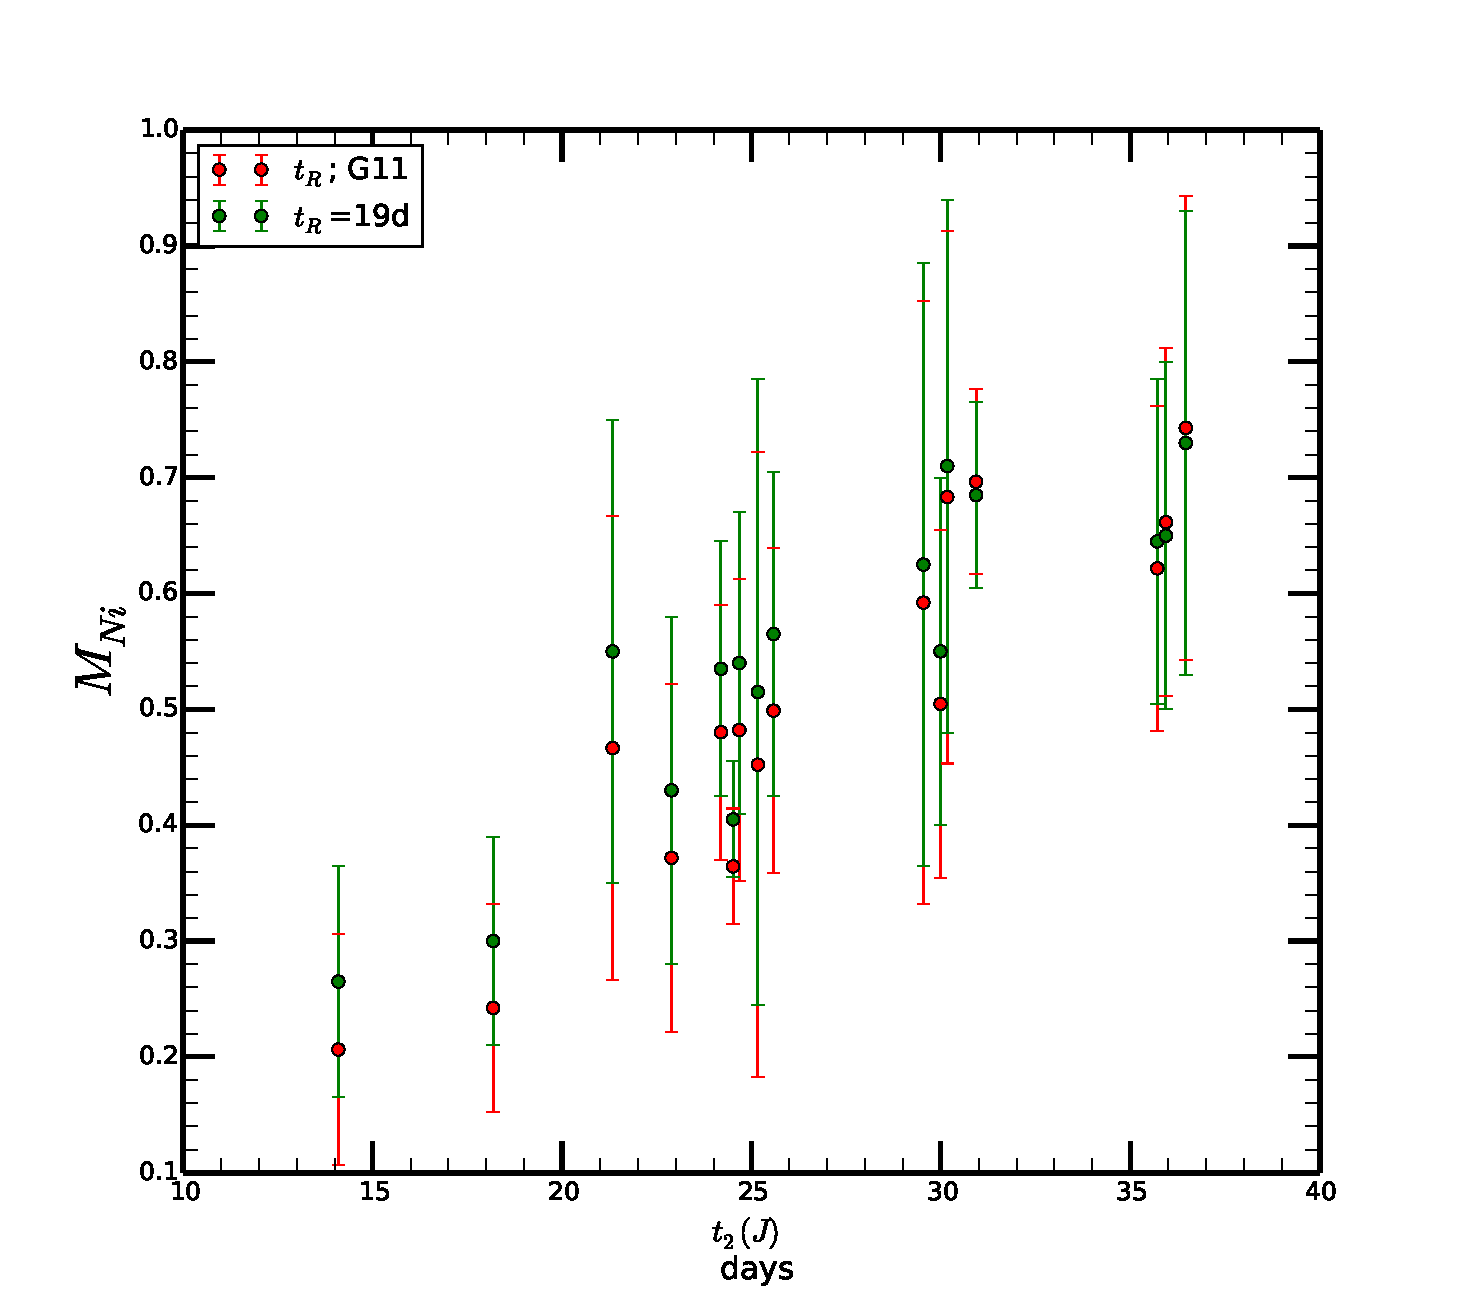
\includegraphics[width=.5\textwidth, trim= 0 30 0 30]{../plot_rel/comp_tr_nit2.pdf}
\caption{Comparison of the $M_{^{56}Ni}$ versus $t_2$ relations for using Arnett's rule with variable (\emph{red circles}) and fixed (\emph{green circles}) rise time. }
\end{figure}

%----------------------------------%

\subsubsection{Interpolating using DDC models}
Another possible method for deriving   $M_{^{56}Ni}$ values from $L_{max}$ is by interpolating the relation found from theoretical models between these two quantities. In our analysis, we use the DDC models from \citet{Blondin2013} as another method of obtaining $M_{^{56}Ni}$.

For objects without NIR coverage, these models can be used to calculate the $M_{^{56}Ni}$-$L_{max}$ relationship for a set of optical-only filters (eg. SN2004gu only has $BVRI$ coverage near maximum). 
This method, therefore, has the advantage of being able to derive $M_{^{56}Ni}$ values for objects with missing passbands without an additional correction term applied to the $L_{max}$. However, in order to keep the samples uniform across the different methods, we only use the objects with complete coverage from $u$ ot $H$ bands. 

%----------%

\begin{figure}
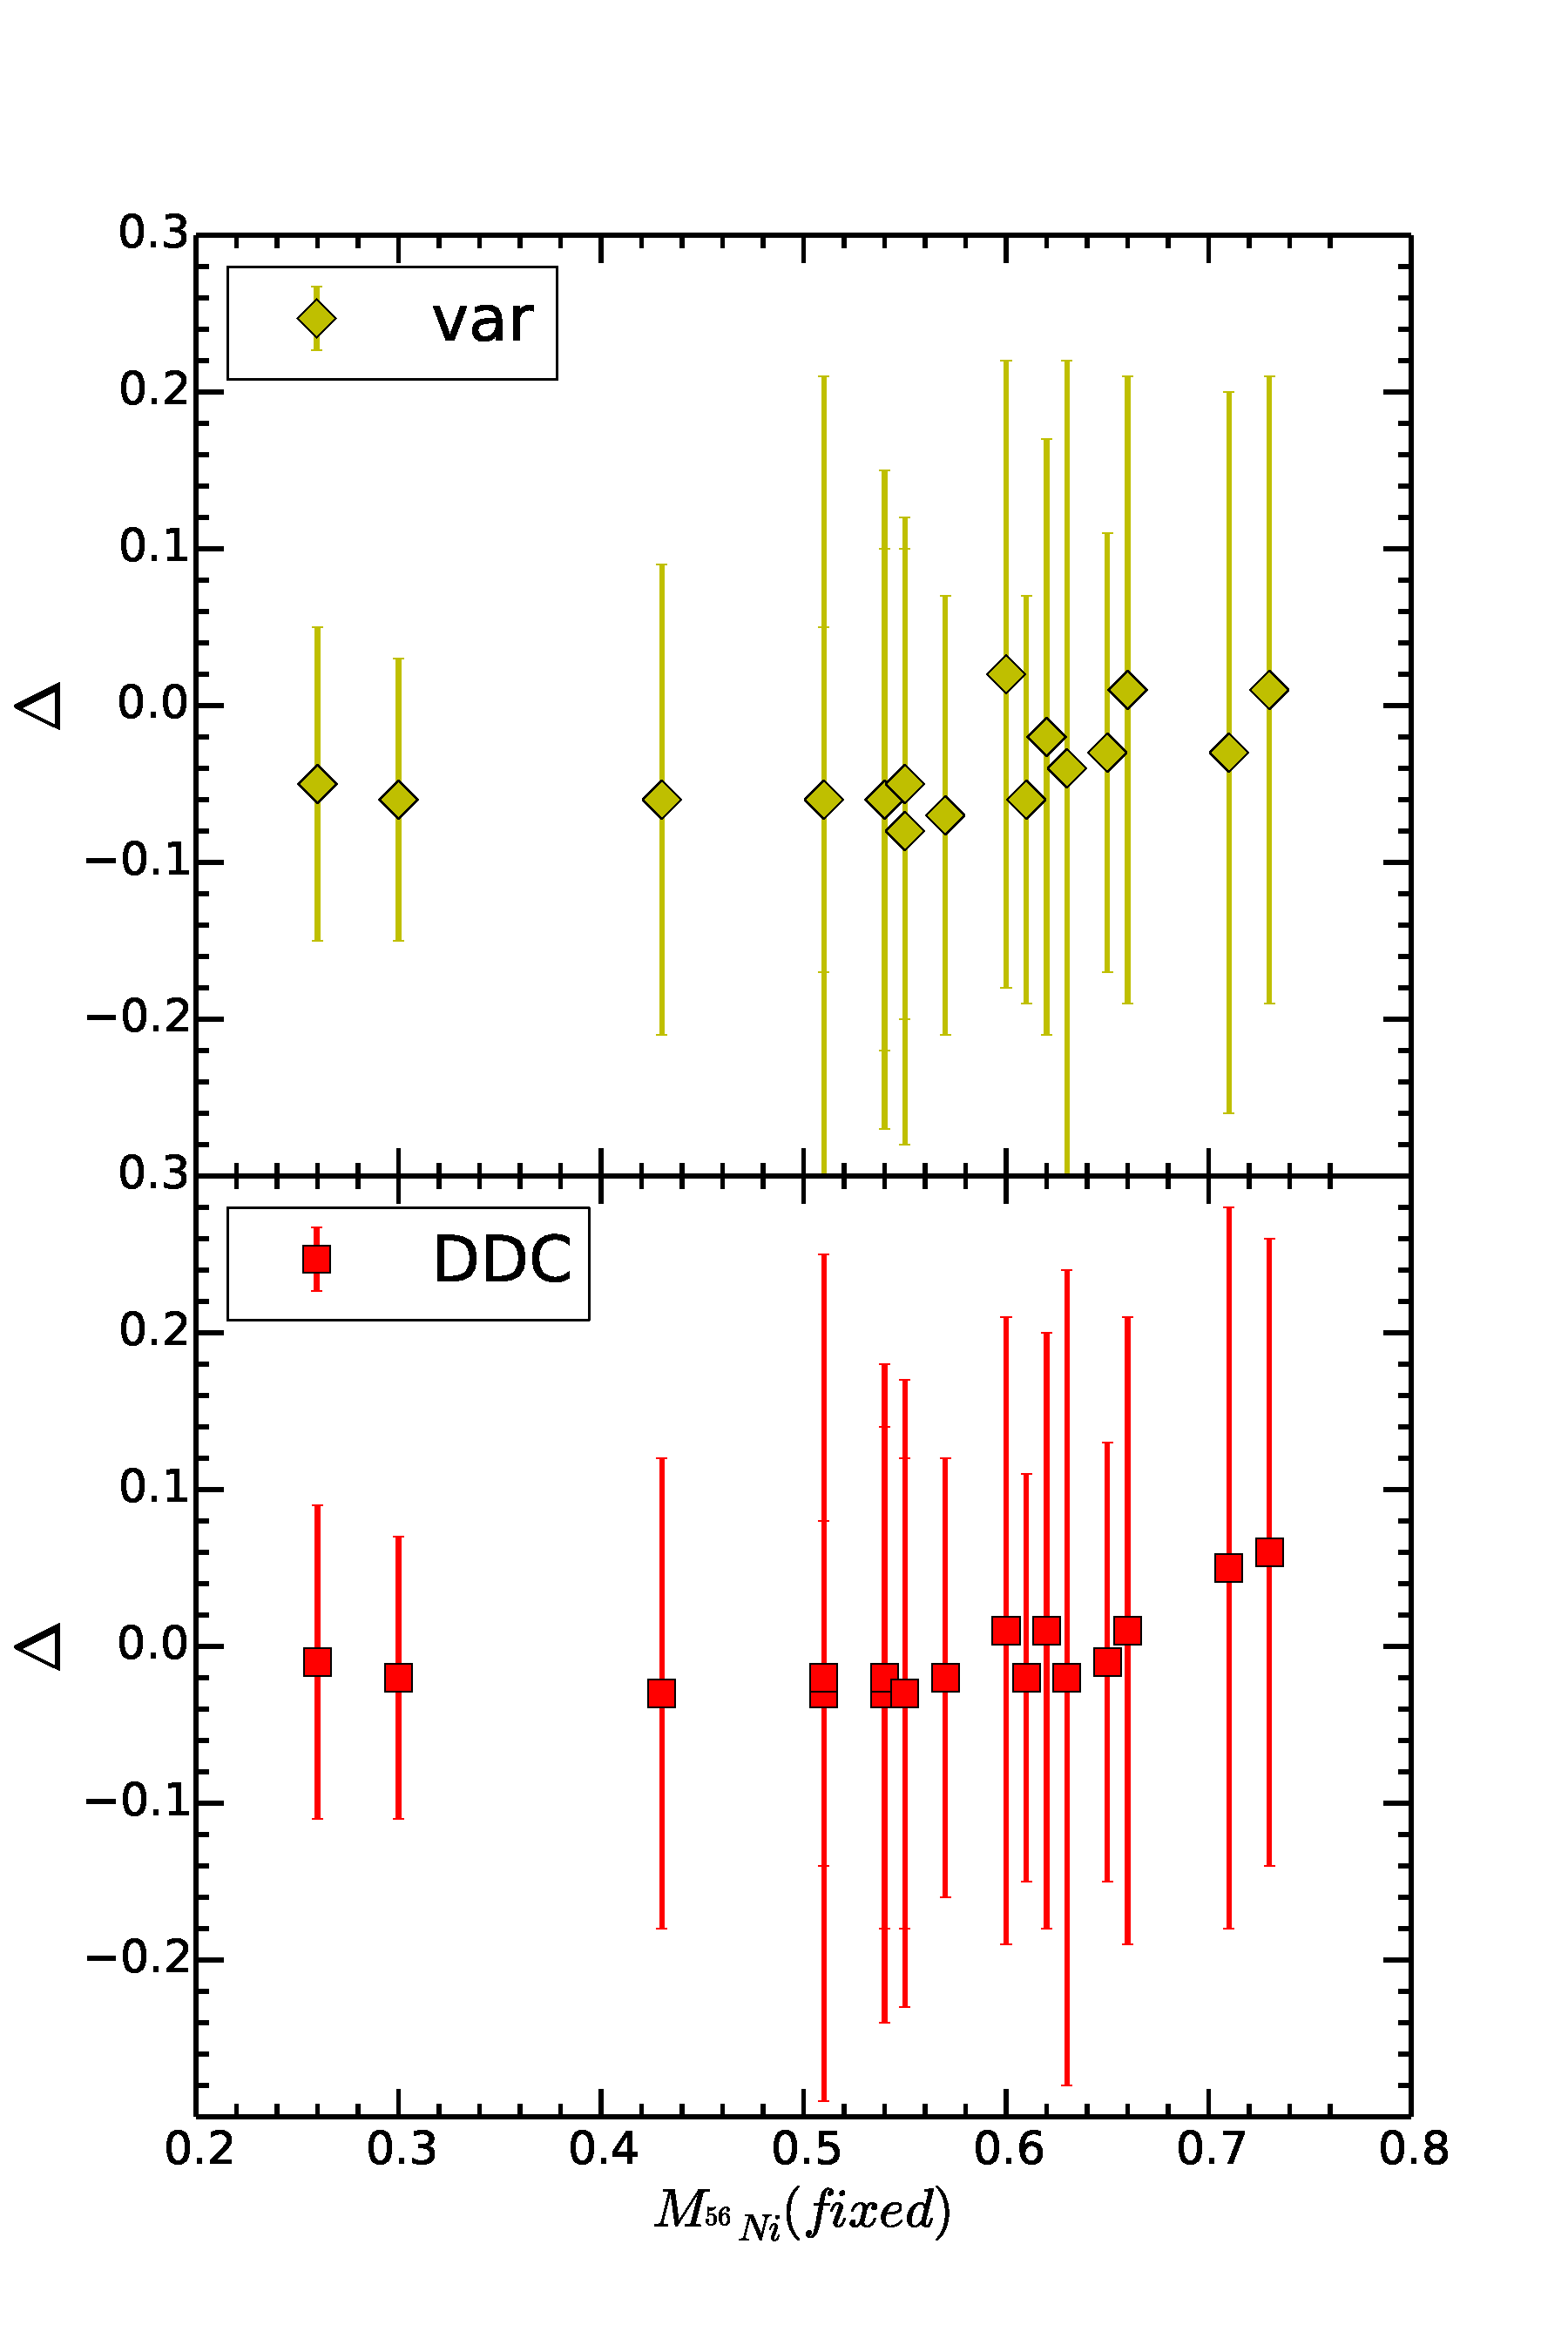
\includegraphics[width=.5\textwidth, trim= 0 30 0 30]{../plot_rel/dif_ni_comp.pdf}
\caption{\emph{Top}: The difference between the values estimated using a fixed rise time with Arnett's rule and the DDC models is plotted against the estimates from Arnett's rule with fixed rise time. \emph{Bottom}: The difference between values estimated using a fixed rise time with Arnett's rule and a variable rise time plotted against the estimates from Arnett's rule with fixed rise time. From the two panels we can see that the difference in the individual measurements are much smaller than the errors from a given method}
\label{fig:difarn}
\end{figure}

%---------------% 

\begin{figure}
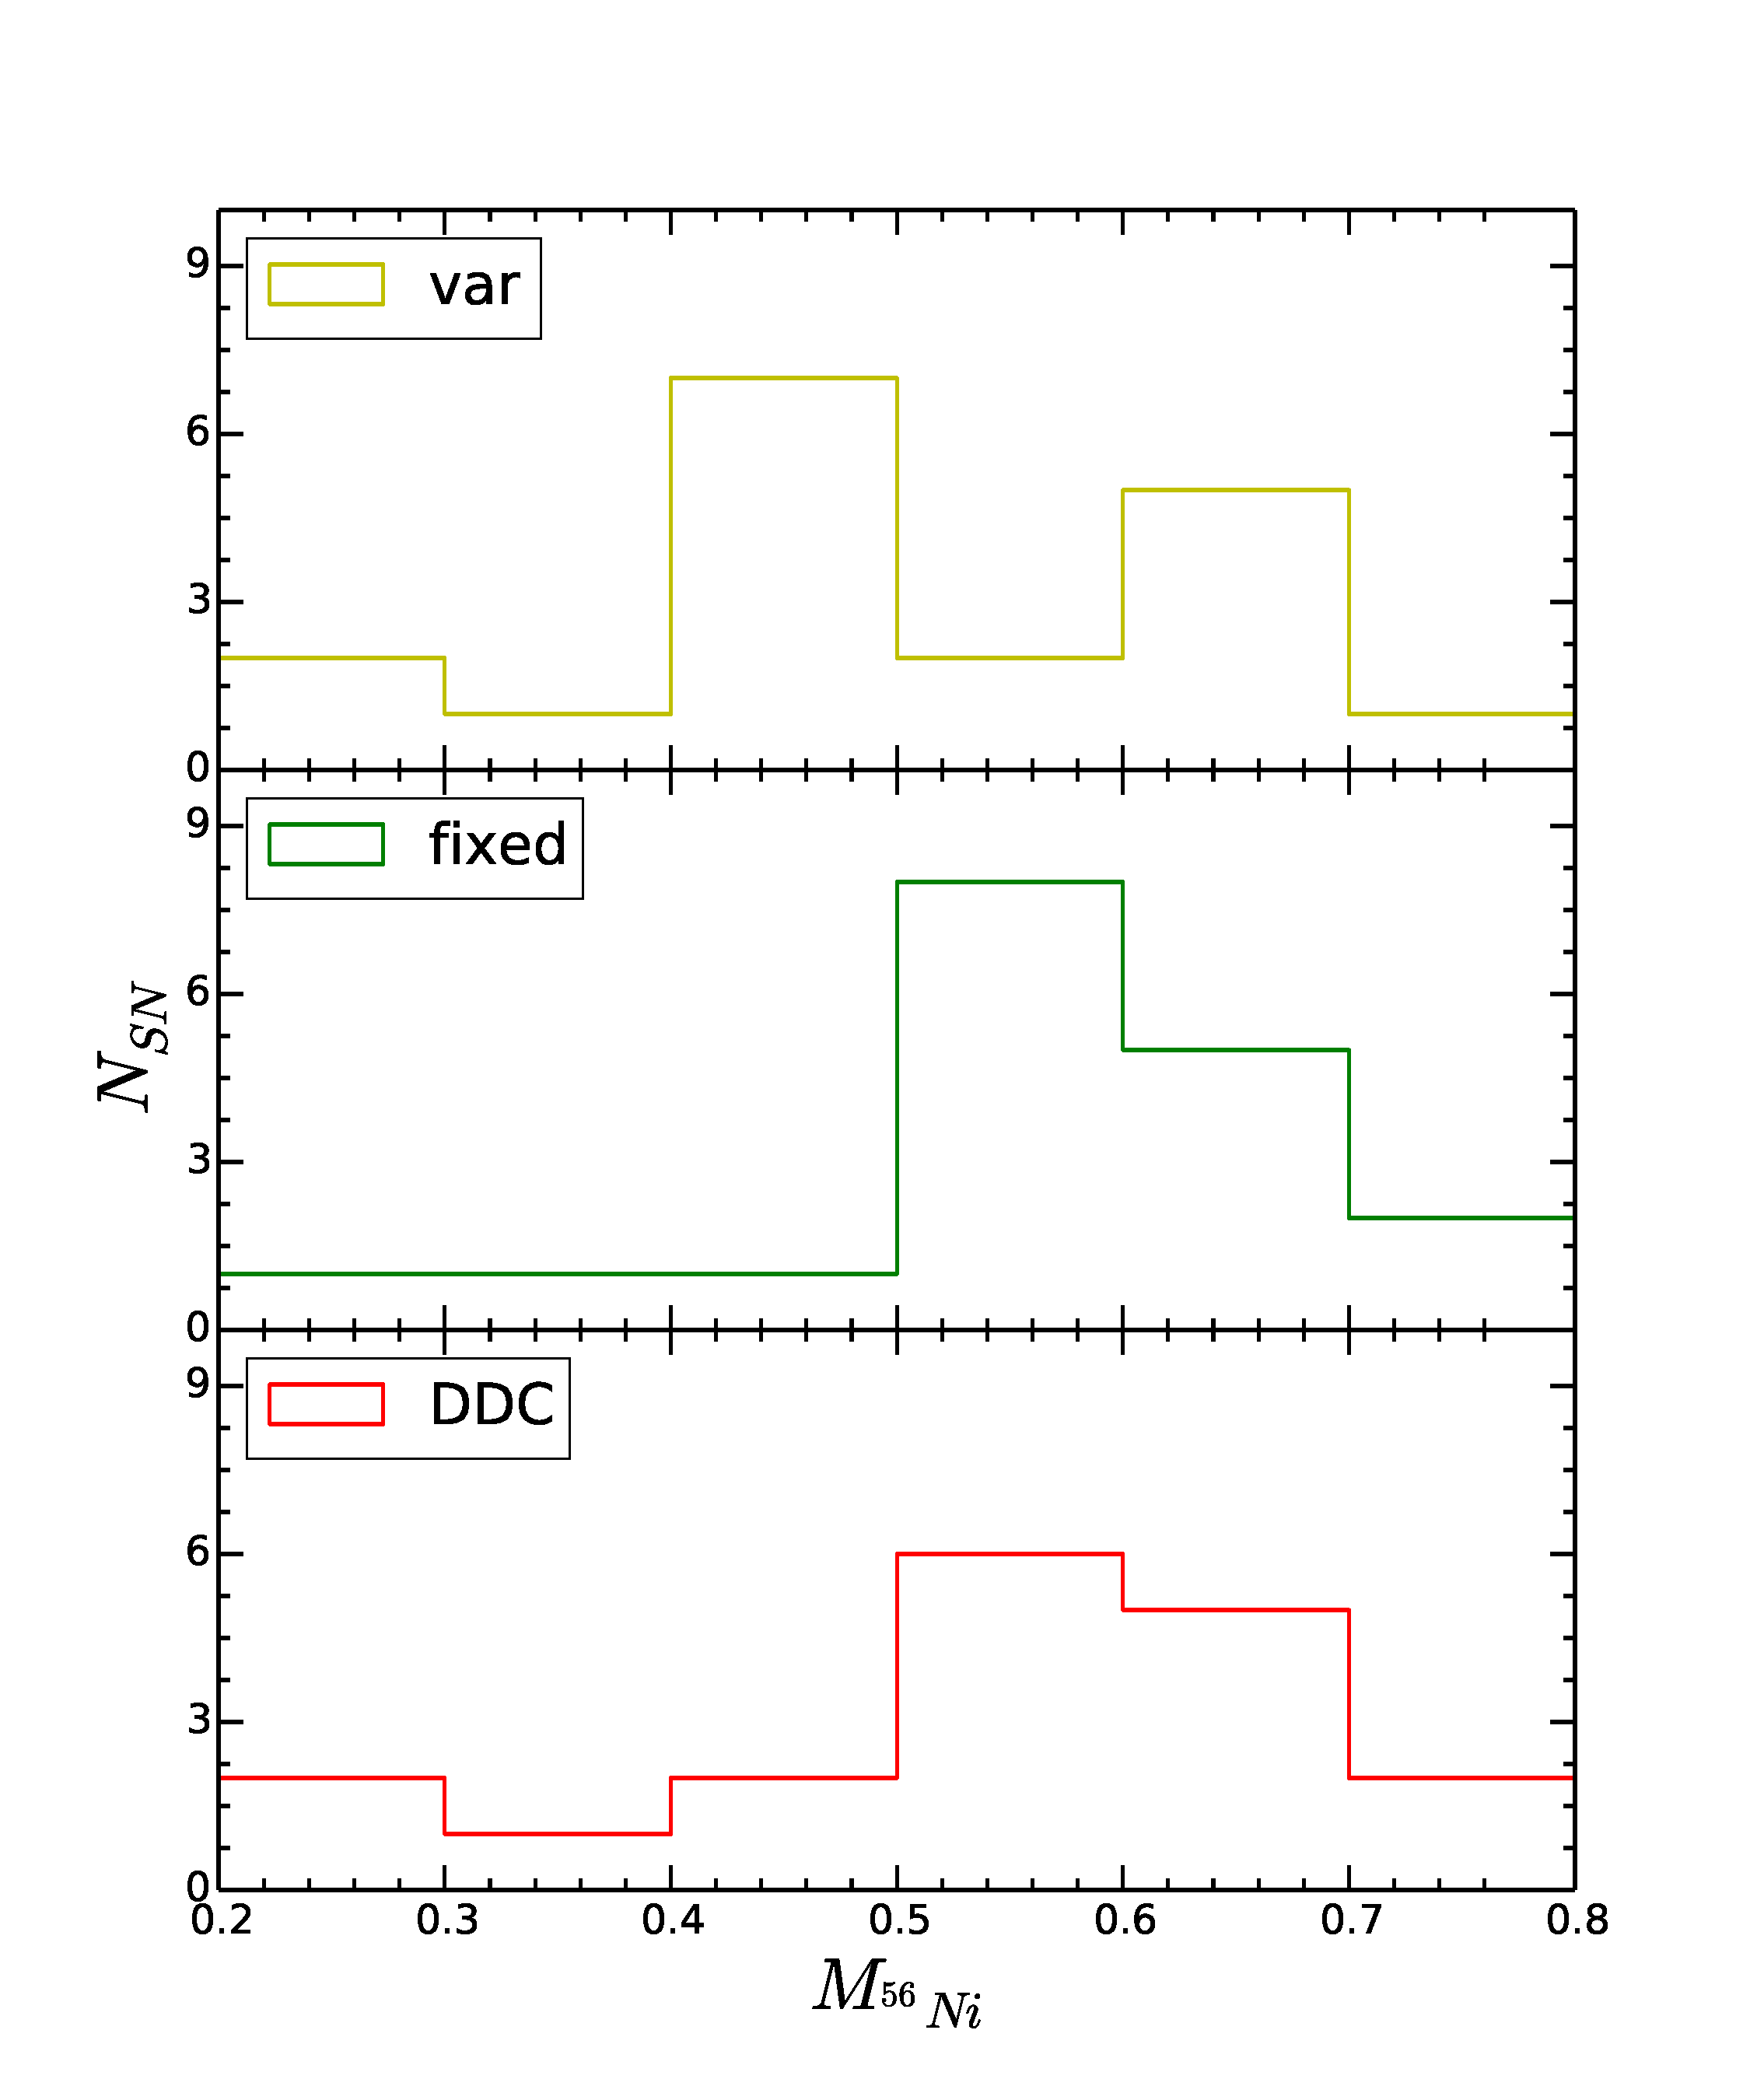
\includegraphics[width=.5\textwidth, trim= 0 30 0 30]{../plot_rel/hist_ni.pdf}
\caption{The histograms show the different methods to estimate the $M_{^{56}Ni}$ from the $L_{max}$. The values from Arnett's rule with fixed and variable rise time are plotted in the \emph{top} and \emph{middle} panels. The \emph{bottom} panel has the values estimated from the DDC models}
\label{fig:nicomp}
\end{figure}


Similar to previous studies we find that there is a large distribution in the $M_{^{56}Ni}$ values for the sample in Table \ref{tab:lr}. We note a factor of $\sim$ 3 difference between the lowest and highest $M_{^{56}Ni}$ values. We note that this sample doesn't include faint, 91bg-like objects, since their NIR light curves don't show a second maximum. These objects are seen to have a much lower $M_{^{56}Ni}$ $\sim$ 0.1 $M_{\odot}$. Thus, the complete distribution of $M_{^{56}Ni}$ for SNIa is expected to be wider than is seen in our sample.

%------------%


\subsection{Test Case for heavily reddened SNe}
Using the correlations derived above, we want to estimate the Ni masses of heavily reddened SNae. The first test case is the nearby SN 2014J in M82 with an $E(B-V)_{host}$ of 1.3. 
Current attempts to use the bolometric light curve depend on the $A_V$ value used and vary by a factor of $\sim$ 2
 (0.37 $M_{\odot}$ if using $A_V$=1.7 mag from \citet{Margutti2014}, compared to 0.77 using a higher $A_V$ of 2.5 mag from \citet{Goobar2014}).  In our analyses the aim is to 
 estimate the $M_{^{56}Ni}$ independent of the extinction.

The proximity of SN2014J, has allowed for the first $\gamma$ ray Co line detection in an SNIa (Churazov+ 2014). the authors, using a line photon escape fraction from the models, 
deduce an Ni mass of 0.62  $\pm$ 0.13 $M_{\odot}$. This provides a direct measurement of  $M_{^{56}Ni}$ for the SN. However, $\gamma$ ray detections aren't possible for farther away SN, for which we require a different estimation method. 

Using the best fit relation for the sample defined above , we obtain $M_{^{56}Ni}$ of 0.66 $\pm$ 0.15 $M_{\odot}$  for a $t_2$ of 31.99 $\pm$ 1.15 days. 
Thus, we find a very good correspondence between the values from the $\gamma$ rays and the NIR second maximum. This adds evidence to the argument that the NIR can be used for estimate $M_{^{56}Ni}$ for highly reddened SN.

Since we find from the DDC models that $\alpha$ is not constant for different $M_{^{56}Ni}$ (and hence, $L_{max}$) values, we use $\alpha$ corresponding to the peak luminosity of SN2014J. We do not find a significant change in the estimated $M_{^{56}Ni}$. Hence, for further analyses, we use $\alpha$=1

\begin{table*}
\begin{center}
\caption{Comparison of different methods to estimate $M_{^{56}Ni}$ for SN2014J}
\begin{tabular}{llcrr}
\hline
 $M_{Ni}$ (inferred) & $\sigma$ & Method & Reference\\
\hline
0.62	& 0.13 & $\gamma$ ray lines & \citet{Churazov2014} \\
0.37	& -- & Bolometric light curve $A_V$=1.7 mag &  \citet{Churazov2014, Margutti2014} \\
0.77	& -- & Bolometric light curve $A_V$=2.5 mag & \citet{Churazov2014, Goobar2014} \\
0.64	& 0.12 & NIR second maximum & this work \\

\hline
\end{tabular}
\end{center}
\label{tab:meth}
\end{table*}


For SN2014J, we can get a precise measurement of the extinction from IR spectra at $\sim$ +300 days ({\bf explain in greater detail}). This is again not possible for 
objects farther away. Thus, we apply this relation to a farther away, heavily extinguished object, SN2006X. 
The measured value for SN2006X of $t_2(J)$ is 28.19 with an error of 0.49  days. This results in an $M_{^{56}Ni}$ value of 0.58 $\pm$ 0.13 $M_{\odot}$. This value is consistent with the conclusion that SN2006X is a 'normal' SNIa \citep{Wang2008}. We compare this value for SN2006X to that obtained using $t_2(Y)$ and obtain $M_{^{56}Ni}$ of 0.58 $\pm$ 0.14 $M_{\odot}$. We find both these values consistent with each other. The slightly higher error bar on
 the value from $t_2(Y)$ is due to a larger error on the 
intercept in the best fit relation for the $Y$ band. 


In \citet{Wang2008}, the authors use multi-band photometry to correct the light curves for absorption from host galaxy dust. They derive a bolometric peak luminosity of 1.02 ($\pm$ 0.1) $\cdot e43$ $erg s^{-1}$. From $R$ band photometry, they derive a rise time to $B$ maximum of 18.2 $\pm$ 0.9d. Using this value in the expression for Arnett's rule, they derive a value of $M_{^{56}Ni}$= 0.50 $\pm$ 0.05 $M_{\odot}$. Thus, we conclude that the value derived from $t_2$ is consistent with published  $M_{^{56}Ni}$ values.   


\begin{table*}



\begin{center}
\caption{$M_{Ni}$ estimates for 5 objects with high values of $E(B-V)_{host}$. We present constraints from the relation using only $t_2(J)$ as well as from both $t_2(Y)$ and $t_2(J)$. We can see a marked decrease in the error values when combined constraints are used}
\begin{tabular}{llcccrr}
\hline
SN & $t_2(J)$ & $M_{Ni}$ (inferred) & $\sigma$ & $\mu$ & $e_{\mu}$ & Method \\
\hline
SN1986G	& 16.40 ($\pm$ 1.4)	&	0.32 & 0.10	& 28.01 & 0.12 & $J$ band relation \\
-- & --	& 0.33	& 0.08	&--&--& combined fit \\
SN2005A	& 27.58 ($\pm$ 0.3)	& 0.57	&  0.13 & 34.51 & 0.11  & $J$ band relation \\
-- & -- &	0.57	& 0.11	&--&--& combined fit \\
SN2006X	& 28.19  ($\pm$ 0.5)	& 0.57 & 0.13 &	 30.91 & 0.08 & $J$ band relation \\
-- & -- &	0.58	& 0.11	&--&--& combined fit \\
SN2008fp & 31.03 ($\pm$ 0.3)	& 0.64	& 0.15 & 31.79 & 0.05 & $J$ band relation \\
-- 	- &-- & 0.64	& 0.13	&--&--& combined fit		\\
SN2014J	& 31.99 ($\pm$ 1.2)	& 0.66	& 0.15 &  27.64 & 0.10   & $J$ band relation\\
--	& -- & 0.66  & 0.13 &--&--& combined fit \\
\hline
\end{tabular}

\label{tab:red}

\end{center}




\end{table*}



We include three more objects in the highly reddened SNe sample, namely, 1986G, 2005A and 2008fp. We calculate the $M_{^{56}Ni}$ for these objects in the same way as for SN2014J and SN2006X. We summarise our findings in Table ~\ref{tab:red}.
We can see that 1986G has a lower value of $M_{^{56}Ni}$ than the other objects in the sample. This is consistent with the observed optical decline rate and lower $B$ band luminosity of the SN. Since we find that $t_2$ in both $Y$ and $J$ bands correlates very strongly with the $M_{^{56}Ni}$, we use combined constraints from the relations to obtain an $M_{^{56}Ni}$ estimate.

% We can see from Table ~\ref{tab:red} that the error on the $M_{^{56}Ni}$ reduces when using combined constraints. For 2014J, it is 0.17 $M_{\odot}$ whereas for the others it is much lower at 0.07 $M_{\odot}$ 


Hence, we conclude that the NIR second maximum timing (in $Y$ and $J$) is a very good indicator of the amount of Nickel synthesised in the explosion, even for heavily reddened objects. 


\subsubsection{Combined fit}
From our analyses, we've found that the $t_2$ in $Y$ and $J$ is very strongly correlated to the $L_{max}$. In table \ref{tab:coeff}, we see that the slope values for the two bands is nearly identical and the intercepts are within the error bars. This prompted us to combine the information from the two bands for extrapolating the values of $L_{max}$ for objects not in the 'low-reddening' sample.

For the five objects listed above which have a very high $A_V$, we used the $J$ band relation to obtain an $M_{^{56}Ni}$. We also used a combined fit to the $Y$ and $J$ band data to evaluate the reduction in the error bar. For this, we presume that the $Y$ band estimate is equivalent to the value in the $J$ band, and hence, we calculate the slope and intercept with a greater number of data points, which leads to a reduction in the errors on the parameter estimates.  

\subsection{Complete NIR Sample}
Since we have derived the relation between $L_{max}$ and $t_2$, we evaluate the $L_{max}$ for all objects with a measured $t_2$ independent of the reddening estimates.
Since the slope for the relation in the $Y$ and $J$ bands is very similar and the intercepts are within error bars, we take the mean value for the slope and intercepFt as a 'combined' relation. We use the higher error on the intercept (from the $Y$ band) for the combined equation. We then use this to compare the estimates of $L_{max}$ from the $t_2$ in the two bands. In figure \ref{fig:yjcomp}, we plot the difference in the $L_{max}$ from the $t_2$ in $J$ and $Y$ against the $L_{max}$ estimated from $t_2(J)$. The difference in the two estimates is smaller than the error on the measurement. We note that the largest difference is for SN2005na, which has a $t_2(J)$ of 32.59, but a much smaller $t_2(Y)$ of 27.54. However, even for this object, the error is higher than the difference between the measurements   
%and have presented the different ways to obtain the $M_{Ni}$ from the $L_{max}$, we can then use the distribution of $t_2$ for all objects, independent of reddening to obtain a distribution of $M_{^{56}Ni}$ using the relations derived


\begin{figure}
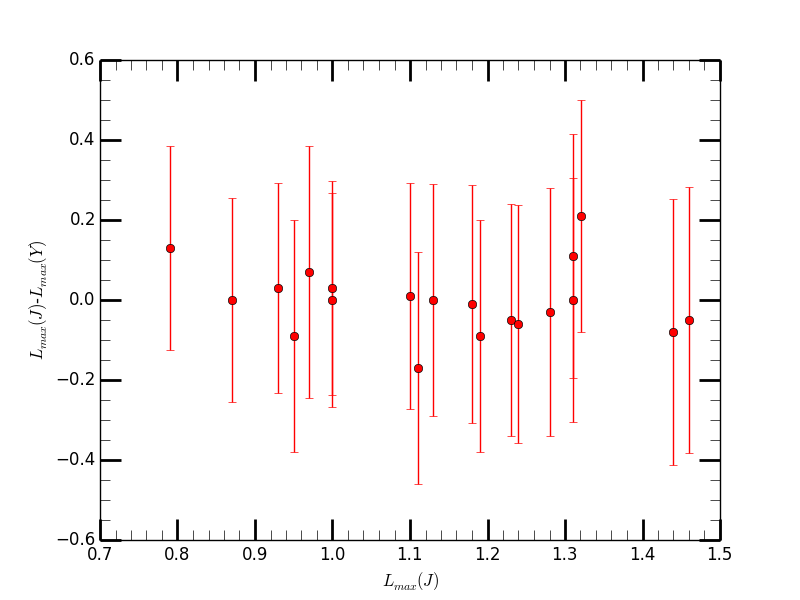
\includegraphics[width=.5\textwidth, height=0.25\textheight, trim= 0 30 0 30]{../plot_rel/lbol_comp_yj.png}


\caption{A comparison of the $L_{max}$ from the $t_2$ values measured in the $Y$ and $J$ bands. Plotted on the x-axis is the $L_{max}$ measured from $t_2(J)$ and on the y-axis is the difference between $L_{max}(J)$ and $L_{max}(Y)$. We can see that there is no trend between the two. The difference has a standard deviation of 0.08 ($\cdot$ $1e^{43}$) $erg s^{-1}$. The errors on each are errors in the individual measurements added in quadrature. We can see that the difference is smaller than the error. }
\label{fig:yjcomp}
\end{figure}

In section \ref{ssec-derni}, we have described the different methods for obtaining $M_{^{56}Ni}$ from $L_{max}$. Hence, we can derive a distribution for $M_{^{56}Ni}$ from the evaluated $L_{max}$ for the complete sample. 
\begin{figure}
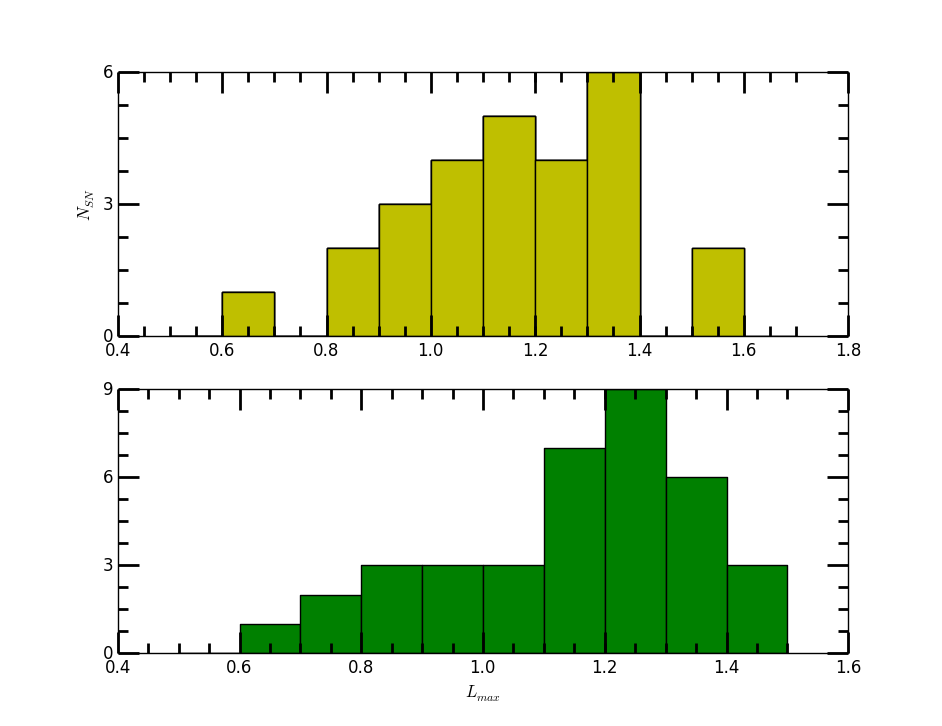
\includegraphics[width=.5\textwidth, trim= 0 30 0 30]{../plot_rel/lbol_yj_compsamp.png}
\caption{Histogram distributions of $L_{max}$ derived from the relations for the complete sample of objects (without the low reddening sample). \emph{Top}: Using the $t_2(Y)$ and \emph{bottom}: Using the $t_2(J)$. A large distribution in the $L_{max}$ values can be seen}
\label{fig:hist}
\end{figure}


In figure \ref{fig:hist} we plot the distribution of $M_{^{56}Ni}$ calculated from the $L_{max}$. We use Arnett's rule with a fixed rise time to get the $M_{^{56}Ni}$ from the $L_{max}$. From figure \ref{fig:hist}, we find a large scatter in the $M_{^{56}Ni}$ values. We find that the objects vary by a factor of 3 in their $M_{^{56}Ni}$ distribution. We note, however, that since faint, 91bg-like objects do not show a second maximum, we do not have values in the figure $\lesssim$ 0.2 $M_{\odot}$, hence, the expected variation for the complete population of SNIa is greater.  


\begin{table}
\begin{minipage}{70mm}
\begin{center}
\footnotetext{$^a$:$\cdot e^{43} erg s^{-1}$}
\caption{$M_{Ni}$ measurements for the complete sample of objects with $t_2$ measurements in both $Y$ and $J$ bands.}
\begin{tabular}{llcrr}
\hline
SN & $L_{max}^{a}$ (J)	& $\sigma$ & $L_{max}^{a}$ (Y) & $\sigma$ \\
\hline
1980N & 0.91 & 0.13 &\ldots & \ldots \\
1981B & 1.32 & 0.15 &\ldots & \ldots\\
1986G & 0.64 & 0.09 &\ldots & \ldots\\
1998bu & 1.23 & 0.14 &\ldots & \ldots\\
1999ac & 1.12 & 0.14 &\ldots & \ldots\\
1999ee & 1.42 & 0.16 &\ldots & \ldots \\
2000E & 1.31 & 0.16 &\ldots & \ldots\\
2000bh & 1.37 & 0.15 &\ldots & \ldots\\
2001bt & 1.17 & 0.13 &\ldots & \ldots\\
2001cn & 1.24 & 0.14 &\ldots & \ldots\\
2001cz & 1.40 & 0.16 &\ldots & \ldots\\
2001el & 1.29 & 0.15 &\ldots & \ldots\\
2002bo & 1.12 & 0.13 &\ldots & \ldots\\
2003cg & 1.24 & 0.14 &\ldots & \ldots\\
2003hv & 0.92 & 0.12 &\ldots & \ldots \\
2004ey	&	1.21	&	0.19	&	1.31	&	0.20	\\
2004gs	&	0.93	&	0.16	&	0.91	&	0.16	\\
2004gu	&	1.46	&	0.22	&	1.54	&	0.22	\\
2005A	&	1.10	&	0.18	&	1.12	&	0.18	\\
2005al	&	1.05	&	0.18	&	1.04	&	0.18	\\
2005na	&	1.35	&	0.20	&	1.13	&	0.19	\\
2006D	&	1.05	&	0.18	&	1.01	&	0.18	\\
2006X	&	1.13	&	0.18	&	1.13	&	0.19	\\
2006ax	&	1.32	&	0.20	&	1.36	&	0.21	\\

2006et	&	1.33	&	0.22	&	1.35	&	0.20	\\
2006gt 	& 0.85 		& 0.11 &\ldots & \ldots\\
2006hb	&	0.79	&	0.17	&	0.72	&	0.15	\\
2006kf	&	1.01	&	0.17	&	1.07	&	0.10	\\
2007S	&	1.46	&	0.21	&	1.52	&	0.23	\\
2007af	&	1.22	&	0.19	&	1.23	&	0.19	\\
2007as	&	1.02	&	0.22	&	0.94	&	0.17	\\
2007bc  &\ldots & \ldots & 1.16 &  0.2 \\
2007bm	&	1.15	&	0.17	&	1.32	&	0.20	\\
2007ca  &\ldots & \ldots & 1.38 &  0.22 \\
2007if  &\ldots & \ldots & 1.34 & 0.22 \\
2007jg  &\ldots & \ldots & 1.12 & 0.2  \\
2007le	&	1.27	&	0.20	&	1.31	&	0.20	\\
2007nq	&	0.98	&	0.18	&	0.94	&	0.17	\\
2008C	&	1.33	&	0.21	&	1.23	&	0.19	\\
2008fp	&	1.28	&	0.20	&	1.33	&	0.21	\\
2014J & 1.32 & 0.18 &\ldots & \ldots \\
\hline
\end{tabular}
\end{center}
\end{minipage}
\label{tab:yj}
\end{table}


In table \ref{tab:comp_ni}, we present the  $M_{^{56}Ni}$ values for the complete sample of objects with a measured $t_2(J)$ value. 




\iffalse
\begin{figure}
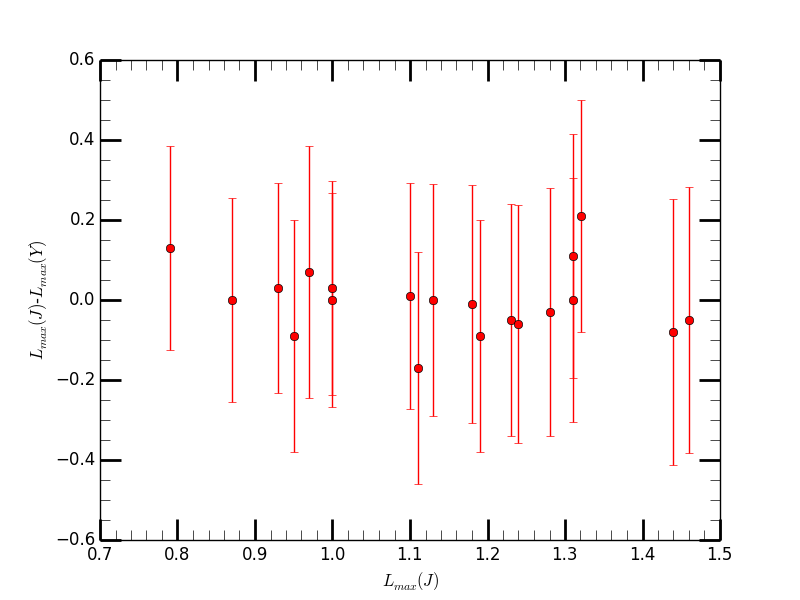
\includegraphics[width=.5\textwidth, trim= 0 30 0 30]{../plot_rel/lbol_comp_yj.pdf}
\caption{The plot shows the difference in the $M_{^{56}Ni}$ measured using $Y$ and $J$ band data, plotted against the $M_{^{56}Ni}$ measured from the $J$ band data. The mean value of the difference is 0.03 $M_{\odot}$ with a standard deviation of 0.037 $M_{\odot}$ (error bars on the x-axis have not been plotted for better visibilty of points)}
\label{fig:yjcomp}
\end{figure}
\fi

In figure \ref{fig:yjcomp}, we plot the difference between the $L_{max}$ estimated from the $t_2$ in $Y$ and $J$ bands against the $L_{max}$ estimated from $t_2(J)$ (called $L_{max}(J)$ in the figure). We find that there is no relation between the two quantities. The mean difference is 0.06 $M_{\odot}$ with a standard deviation of 0.05 $M_{\odot}$. This is lower than the error estimate on the individual values, which can be seen in the figure. 	


\subsection{Comparison with published values}
We searched the literature for published values of $M_{^{56}Ni}$ for objects in our sample. In \citet{Scalzo2014} , the authors published values of $M_{^{56}Ni}$ for 2005el and 2011fe. For 2011fe, we find $M_{^{56}Ni}$ of 0.52 $\pm$ 0.15 $M_{\odot}$ whereas the value in S14 is 0.42 $\pm$ 0.08. We note that the value of $\alpha$ in their study is 1.2 whereas we use $\alpha$=1. Using their value of $\alpha$, we find $M_{^{56}Ni}$= 0.44 $M_{\odot}$, which is a better agreement. SN2011fe also has a publsihed $M_{^{56}Ni}$ value in \cite{Pereira2013}, where the authors use different values of $\alpha$. For $\alpha$=1 they report a value of 0.53 $\pm$ 0.11 $M_{\odot}$, which agrees well with the value in this work. 

For SN2005el we find $M_{^{56}Ni}$ of 0.46 $\pm$ 0.11 $M_{\odot}$. S14 provides a discussion of this object, which in their sample they measure to have an  $M_{^{56}Ni}$ of 0.52. It is one of two outliers in their $M_{^{56}Ni}$-$\Delta m_{15}$. They argue that it is likely for the SN to have a lower $M_{^{56}Ni}$ that their fiducial analysis suggests.  






























\section{Discussion and Conclusion}
\label{sec-dnc}
In our sample, we observe a strong correlation between the $M_{Ni}$ and $t_2$ in $Y$ and $J$, and less so in the $H$ band. 
This provides us with direct evidence that the timing of the second maximum is governed by the amount of Nickel produced by the supernova
since it leads to a later ionization transition of the iron group elements at late time (mainly, $^{56}Co$) from doubly to singly ionized \citep{Kasen2006}.

This trend is confirmed by a strong correlation between  $t_L$  and $M_{Ni}$ indicating that objects with more Ni produced have a slower
rate of reddening and the Fe and Co lines appear later in the spectrum, which delays the onset of the lira law phase, and also the second maximum.

This relation offers great insight into measuring the $M_{Ni}$ for objects not in the low-reddening sample, but with extensive NIR data. 
A striking example of this application is the nearby SN2014J in M82, which is heavily occluded by host galaxy dust. Since this prevents 
an accurate measurement of $M_{Ni}$ from the bolometric light curves and there is a large disparity in the different values published in the literature
using this method, we use the relations we obtain to constrain the $M_{Ni}$. For SN2014J, we have a unique opportunity to compare different estimation methods, 
since its proximity has allowed $\gamma$ ray Co line detection and therefore, another extinction independent measurement of the $M_{Ni}$. Our value of 0.58 $\pm$ 0.21 $M_{odot}$
compares very well with \citet{Churazov2014}, who find $M_{Ni}$ of 0.61 $\pm$ 0.13 $M_{odot}$. The brightness of SN2014J at late times, due to its proximity, permits us to obtain
NIR spectra at $\sim$ 300 days, which can provide an accurate measurement of the extinction and therefore, an accurate $M_{Ni}$ from the bolometric light curve. This presents
us with a confrontation of several different methods to measure the $M_{Ni}$ and hence obtain a conclusive estimate on the amount of Ni produce in this SN.

Since $\gamma$ detections are unlikely for farther out SN and most of them are too faint at $\sim$ +300 days for IR spectroscopy, we apply our method to other heavily reddened SN
that are farther away than SN2014J. The first object we analyse is SN2006X. From the measurement of 0.57 $\pm$ 0.15 $M_{odot}$, we conclude that
2006X produced the average amount of Ni for an SNIa.

We also analyse the bolometric light curves at peak and during the late phase of exponential decline. We find that the SN in our sample have a uniform 
late time bolometric decline rate, indicating that the internal structure of the ejecta is similar for most SN. This confirms the deductions from the optical and NIR 
light curves in previous studies and from the bolometric light curves in sample of C00. We also find that the bolometric light curves, unlike the optical light curves,
have a narrow distribution of the $\Delta m_{15}$ parameter.  

We conclude from our findings that there is a strong dependence of the $t_2$ and the colour evolution (parametrized by $t_L$) on the $M_{Ni}$
\section{To add}
1. $t_l$ versus $M_{Ni}$ plot


2. $M|_{55}$ versus Ni mass in all 3 filters


3. add columns to table \ref{tab:mni} with t2 values so that all params are in one set.



4. possibly add ejecta masses too, depending on the point the paper is making

\iffalse
\section{Infrared Light Curve Morphology}
\label{sec-LC}
\input{sec_max_v10.tex}

\section{Correlations}
\label{sec-corr}
\input{corr_v10.tex}

\section{Discussion}
\label{sec-disc}
\input{discussv10.tex}

\section{Conclusions}
\input{conc.tex}
\label{sec-conc}
\fi



\begin{acknowledgements}
This research was supported by the DFG cluster of excellence ʻOrigin and
Structure of the Universe' We would like to thank Chris Burns for his
help with template fitting using SNooPy, Richard Scalzo for discussion
on the nickel masses and Saraubh Jha on the nature of Type Ia
supernovae. We thank Stephane Blondin for his comments on the manuscript.
B.L. acknowledges support for this work by the Deutsche
Forschungsgemeinschaft through TRR33, The Dark Universe and the Mount
Stromlo Observatory for a Distinguished Visitorship during which most of
this publication was prepared.



\end{acknowledgements}
\iffalse
%\newpage
\begin{thebibliography}{}
%%------------
%

\bibitem[Axelrod (1980)]{axelrod80}
Axelrod, T. S. 1980, PhD Thesis, Univ. of California, Santa Cruz

\bibitem[Candia et al.(2003)]{candia03}
Candia, P., Krisciunas, K., Suntzeff, N. B., et al. 2003, \pasp, 115, 277

\bibitem[Cappellaro et al.(1997)]{cappellaro97}
Cappellaro, E., Mazzali, P. A., Benetti, S., et al. 1997, \aap, 329, 203

\bibitem[Colgate et al.(1980)]{colgate80}
Colgate, S.~A., Petscheck, A.~G., \& Kriese, J.~T. 1980, ApJ, 237, L81

\bibitem[Contardo et al.(2000)]{contardo00}
Contardo, G., Leibundgut, B., \& Vacca, W.~D. 2000, \aap, 359, 876

\bibitem[Elias \& Frogel(1983)]{elias83}
Elias, J. H., \& Frogel, J. A. 1983, \apj, 268, 718

\bibitem[Elias-Rosa et al.(2006)]{eliasrosa06}
Elias-Rosa, N., Benetti, S., Cappellaro, E., et al. 2006, \mnras, 369, 1880

\bibitem[Fransson, Houck \& Kozma(1996)]{fransson96}
Fransson, C., Houck, J., \& Kozma, C. 1996, 
IAU Colloq.~145: Supernovae and Supernova Remnants, 211 

\bibitem[Hawarden et al.(2001)]{hawarden01}
Hawarden, T. G., Leggett, S. K., Letaqsky, M. B., et al. 2001, \mnras, 325, 563

%\bibitem[Kasen et al.(2003)]{kasen03}
%Kasen, D., Nugent, P., Wang, L., et al. 2003, \apj, 593, 788

\bibitem[Kozma et al.(2005)]{kozma05}
Kozma, C., Fransson, C., Hillebrandt, W., et al. 2005, \aap, 437, 983

\bibitem[Krisciunas et al.(2003)]{krisciunas03}
Krisciunas, K., Suntzeff, N. B., Candia, P., et al. 2003, \aj, 125, 166

\bibitem[Krisciunas et al.(2007)]{krisciunas07}
Krisciunas, K., Garnavich, P., Suntzeff, N. B., et al. 2007, \aj, 133, 58

\bibitem[Lair et al.(2006)]{lair06}
Lair, J., Leising, M. D., Milne, P., et al. 2006, \aj, 132, 2024

\bibitem[Landolt(1992)]{landolt92} 
Landolt, A. U. 1992, \aj, 104, 340

\bibitem[Li et al.(2001)]{li01}
Li, W., Filippenko, A. V., Gates, E., et al. 2001, \pasp, 113, 1178

\bibitem[Leibundgut(2001)]{leibundgut01}
Leibundgut, B. 2001, \aapr, 39, 67

\bibitem[Leggett et al.(2006)]{leggett06}
Leggett, S. K., Currie, M. J., Varricatt, W. P., et al. 2006, \mnras, 373, 781
\bibitem[Mattila et al.(2005)]{mattila05}
Mattila,  S., Lundqvist, P., Sollerman, J., et al. 2005, \aap, 443, 649

\bibitem[Milne et al.(1999)]{milne99}
Milne, P.~A., The, L. S., \& Leising, D. 1999, ApJS, 124, 503

\bibitem[Milne et al.(2001)]{milne01}
Milne, P.~A., The, L. S., \& Leising, D. 2001, ApJ, 559, 1019

\bibitem[Monard(2001)]{monard01}
Monard, A. G. 2001, IAU Circ. 7720

\bibitem[Motohara et al.(2006)]{motohara06}
Motohara, K., Maeda, M., Gerardy, C. L., et al. 2006, \apjl, 652, 101 

\bibitem[Ruiz-Lapuente \& Spruit (1998)]{pilar98}
Ruiz-Lapuente, P., \& Spruit, H. 1998, ApJ, 500, 360

\bibitem[Schlegel et al.(1998)]{schlegel98}
Schlegel, D. J., Finkbeiner, D. P., \& Davis, M. 1998, \apj, 500, 525

\bibitem[Sollerman, Leibundgut \& Spyromilio(1998)]{sollerman98}
Sollerman, J., Leibundgut, B., \& , Spyromilio, J. 1998, \aap, 337, 207

\bibitem[Sollerman, Leibundgut \& Lundqvist(2001)]{sollerman01}
Sollerman, J., Leibundgut, B., \& Lundqvist, P. 2001, IAU Cir. 7723 

\bibitem[Sollerman et al.(2004)]{sollerman04}
Sollerman, J., Lindahl, J., Kozma, C., et al. 2004, \aap, 428, 555

\bibitem[Sollerman et al.(2005)]{sollerman05}
Sollerman, J., Cox, N., Mattila, S., et al. 2005, \aap, 429, 559

\bibitem[Spyromilio et al.(2004)]{spyromilio04}
Spyromilio, J., Gilmozzi, R., Sollerman, J., et al. 2004, \aap, 426, 547

\bibitem[Stanishev et al.(2007)]{stanishev07}
Stanishev, V., Goobar, A., Benetti, S., et al. 2007, \aap, accepted

\bibitem[Stritzinger et al.(2006)]{stritzinger06}
Stritzinger, M.~D., Mazzali, P.~A., Sollerman, J., Benetti, S. 2006, \aap,
460, 793


\end{thebibliography}

%table 1 
\clearpage 
\setcounter{table}{0}
\begin{table}
\caption{Log of optical VLT observations for SN~2001el.}
\label{table:1}
\centering
\begin{tabular}{ccccc}
\hline\hline
Phase$^{a}$ & Filter & Exposure & Airmass & Seeing  \\
(days)      &        & (s)      &         & (arcsec) \\
\hline
310        & $U$  & 2$\times$800 & 1.24 & 0.89 \\
310        & $B$  & 3$\times$180 & 1.41 & 0.56  \\
310        & $V$  & 3$\times$150 & 1.32 & 0.62  \\
310        & $R$  & 3$\times$150 & 1.28 & 0.66  \\
310        & $I$  & 3$\times$180 & 1.25 & 0.56  \\
367        & $V$  & 3$\times$300 & 1.23 & 1.16  \\
367        & $R$  & 3$\times$300 & 1.19 & 0.98  \\
367        & $I$  & 3$\times$300 & 1.15 & 1.08  \\
370        & $V$  & 3$\times$300 & 1.08 & 0.60  \\
370        & $R$  & 3$\times$300 & 1.19 & 0.60  \\
370        & $I$  & 3$\times$300 & 1.11 & 0.60  \\
398        & $U$  &2$\times$1020 & 1.36 & 1.00 \\
398        & $B$  & 3$\times$300 & 1.26 & 0.78 \\
430        & $U$  & 1$\times$790 & 1.07 & 1.02 \\ %not detectable sne
430        & $V$  & 3$\times$600 & 1.11 & 0.80 \\
430        & $R$  & 3$\times$720 & 1.25 & 1.00 \\
436        & $B$  & 3$\times$600 & 1.07 & 0.84 \\
436        & $R$  & 3$\times$720 & 1.07 & 1.20 \\
436        & $I$  & 6$\times$900 & 1.19 & 1.00 \\
437        & $U$  &3$\times$1020 & 1.20 & 1.00\\ %no sne
437        & $R$  & 3$\times$720 & 1.11 & 0.80 \\
\hline
\end{tabular} \\
\begin{tabular}{lll}
$^a$ Refers to days past $B_{\rm max}$. && \\
\end{tabular}
\end{table}

%table 2
\setcounter{table}{1}
\begin{table}
\caption{Magnitudes for local standards in the optical.}
\label{table:2}
\centering
\begin{tabular}{rrccccc}
\hline\hline
Offsets$^a$ & & $U$ & $B$ & $V$ & $R$ & $I$ \\
\hline
181.6 N & 72.8 E  & 20.50(0.08)$^b$  & 20.68(0.05) & 20.13(0.05) & 19.78(0.06) & 19.43(0.05) \\
193.6 N & 61.6 E  & 19.84(0.08)      & 19.84(0.05) & 19.18(0.05) & 18.77(0.06) & 18.40(0.05) \\
179.2 N & 56.8 W  & 20.66(0.08)      & 20.66(0.05) & 20.00(0.05) & 19.59(0.06) & 19.21(0.05) \\
6.4   N & 113.6 W & 20.42(0.08)      & 20.33(0.05) & 19.61(0.05) & 19.19(0.06) & 18.80(0.05) \\
56.8  S & 99.2 W  & 22.44(0.09)      & 21.41(0.05) & 19.73(0.05) & 18.70(0.06) & 17.60(0.05) \\
62.4 S  & 95.2 W    & 22.73(0.10)      & 22.69(0.05) & 22.01(0.05) & 21.66(0.06) & 21.32(0.06) \\
72.8 S  & 140.0 W & 19.51(0.08)      & 19.67(0.05) & 19.18(0.05) & 18.86(0.06) & 18.54(0.05) \\
73.6 N  & 181.6 E & 20.73(0.08)      & 21.10(0.05) & 21.02(0.05) & 20.92(0.06) & 20.71(0.05) \\
39.2 S  & 136.8 E & \nodata          & 21.57(0.05) & 20.09(0.05) & 19.19(0.06) & 18.33(0.05) \\
132.0 S & 22.4 W  & \nodata          & 23.18(0.05) & 21.62(0.05) & 20.67(0.06) & 19.68(0.05) \\
\hline
\end{tabular} \\
\begin{tabular}{lll}
$^a$ Offsets in arcseconds measured from the supernova. && \\
$^b$ Numbers in parentheses are uncertainties. && \\
\end{tabular}
\end{table}

\setcounter{table}{2}
%table 3
\begin{table}
\caption{Log of near-infrared VLT observations for SN~2001el.}
\label{table:3}
\centering
\begin{tabular}{ccccc}
\hline\hline
Phase$^{a}$ & Filter & Exposure$^b$ & Airmass & Seeing  \\
(days)      &        & (s)      &         & (arcsec) \\
\hline
316        & $H$     &   10$\times$6$\times$25 & 1.13 & 0.49 \\
316  & $K_{s}$ &   10$\times$6$\times$28 & 1.30 & 0.41 \\
317        & $J$     &   30$\times$4$\times$24 & 1.18 & 0.52 \\
370        & $J$     &   30$\times$4$\times$23 & 1.06 & 0.65 \\
370        & $H$     &   10$\times$6$\times$17 & 1.15 & 0.44 \\
370        & $K_{s}$ &   10$\times$6$\times$30 & 1.08 & 0.40 \\
%383        & $J$     &   30$\times$4$\times$18 & 1.23 & 0.61 \\
383        & $K_{s}$ &   10$\times$6$\times$20 & 1.11 & 0.40 \\
443        & $H$     &   10$\times$6$\times$30 & 1.14 & 0.40  \\
443        & $J$ &   30$\times$4$\times$30 & 1.14 & 0.40 \\
443  & $K_{s}$ &   30$\times$4$\times$27 & 1.09  & 0.60  \\
445        & $J$ &   30$\times$4$\times$23 & 1.17 & 0.70 \\
445        & $H$     &   10$\times$6$\times$60 & 1.06 & 0.55 \\
\hline
\end{tabular} \\
\begin{tabular}{lll}
$^a$ Refers to days past $B_{\rm max}$. && \\
$^b$ Detector integration time (DIT)$\times$number of DITs per exposure$\times$
number of exposures. && \\
\end{tabular}
\end{table}
\clearpage

%table 4
\setcounter{table}{3}
\begin{table}
\caption{Magnitudes for local standards in the near-infrared.}
\centering
\begin{tabular}{llccc}
\hline\hline
Offsets$^a$ &  & $J$ &  $H$ & $K_{s}$ \\
\hline
55.35 N & 11.96 W     &   12.98(0.06)$^{b}$ & 12.57(0.05)  &  12.51(0.05)\\
     41.9 N   &      21.4 W &         17.54(0.06)  &      16.89(0.05)   &  16.09(0.05)\\
17.4 S  & 46.3 W & 13.56(0.06)      & 13.18(0.05) & 13.07(0.05)\\
25.4 S  & 42.3 E & 17.54(0.06)      & 17.24(0.05) & 16.95(0.05)\\
53.9 S  & 24.5 E & 19.36(0.06)      & 18.91(0.06) & 18.75(0.05)\\
50.8 S  & 62.8 E & 16.83(0.06)      & 16.44(0.05) & 16.24(0.05)\\
65.9 S  & 49.4 E & 16.27(0.06)      & 15.83(0.05) & 15.59(0.05)\\
\hline
\end{tabular} \\
\begin{tabular}{lll}
$^a$ Offsets in arcseconds measured from the supernova. && \\
$^b$ Numbers in parentheses are uncertainties. && \\
\end{tabular}
\end{table}

%table5
\setcounter{table}{4}
\begin{table}
\caption{Late-time optical magnitudes of SN~2001el.}
\centering
\begin{tabular}{cccccc}
\hline\hline
Phase$^{a}$ & $U$ & $B$  & $V$ & $R$ & $I$ \\
(days)      &     &      &     &     &     \\
\hline
 310 &21.64(0.09)$^b$  & 20.22(0.05) &  20.04(0.05)  & 20.45(0.06) & 19.68(0.05) \\
 367 & \nodata      & \nodata      &  20.88(0.10)  & 21.16(0.09) & 20.17(0.10) \\
 370 & \nodata      & \nodata      &  20.95(0.04)  & 21.36(0.04) & 20.28(0.03) \\
 398 &22.81(0.14)  & 21.45(0.06) & \nodata       & \nodata      & \nodata      \\
 430 &23.44(0.25)  & \nodata      &  21.81(0.06)  & 22.25(0.16) & \nodata      \\
 436 & \nodata      & 22.03(0.07) & \nodata       & 22.61(0.15) & 20.99(0.08) \\
 437 &23.56(0.31)  & \nodata      & \nodata       & 22.18(0.08) & \nodata      \\
\hline
\end{tabular} \\
\begin{tabular}{lll}
$^a$ Refers to days past $B_{\rm max}$. && \\
$^b$ Numbers in parentheses are uncertainties. && \\
\end{tabular}
\end{table}



%table 6
\setcounter{table}{5}
\begin{table}
\caption{Late-time near-infrared magnitudes of SN~2001el.}
\centering
\begin{tabular}{cccc}
\hline\hline
Phase$^a$ & $J$ & $H$ & $K_{s}$ \\
(days)    &     &     &        \\
\hline
 316 & \nodata          & 18.40(0.12)$^{b}$ &  20.07(0.21)  \\
 317 & 19.15(0.10)      &  \nodata          &  \nodata      \\
 370 & 19.21(0.11)      & 18.62(0.11)       &   19.36(0.42)\\
 383 & \nodata       &  \nodata          &   19.54(0.52) \\
 %442 & \nodata          & 18.96(0.11)       &  \nodata      \\
 443 & 19.55(0.12)      & 18.89(0.11)       &   \nodata      \\
 445 & 19.23(0.12)      & 18. 47(0.12)       &   \nodata       \\
\hline
\end{tabular} \\
\begin{tabular}{lll}
$^a$ Refers to days past $B_{\rm max}$. && \\
$^b$ Numbers in parentheses are uncertainties. && \\
\end{tabular}
\end{table}


%table7
\setcounter{table}{6}
\begin{table}
\caption{Decline rates of late-time light curves$^a$.}
\label{table:7}
\centering
\begin{tabular}{cccccccc}
\hline\hline
$U$ & $B$ & $V$ & $R$ & $I$ & $J$ & $H$ & $K_{s}$ \\
\hline
1.43(0.14) &  1.43(0.06) &  1.48(0.06) &  1.45(0.07) &  1.03(0.07) &  0.19(0.10) &  0.17(0.11) &  -1.04(0.65)\\
\hline
\end{tabular}
\begin{tabular}{lll}
$^a$ Mag per 100 days between 310 and 450 days; errors in parenthesis are $1\sigma$. && \\
\end{tabular}
\end{table}
\fi

\end{document}
 
